% NOTE: switch to elsarticle before submission
\documentclass[11pt]{article}

\usepackage{amsmath,amssymb,mathtools}
\usepackage{graphicx}
\usepackage{booktabs}
\usepackage{longtable}
\usepackage{hyperref}
\usepackage{tabularx}
\usepackage{pdflscape}
\usepackage{array}
\usepackage{caption}
\usepackage{orcidlink}
\usepackage{fancyhdr}

\graphicspath{{fig/}}

% Notation macros
\newcommand{\Epica}{\mathcal{E}}  % PICA enable matrix
\newcommand{\Etauf}{E_{\tau,f}}  % Foundations empirical endomap
\newcommand{\Phat}{\widehat{P}}  % induced macro kernel
\newcommand{\Z}{Z}
\newcommand{\X}{X}

\title{To Create a Stone with Six Birds:\\Emergent Geometric and Thermodynamic Regimes\\from a Minimal Stochastic Substrate}
\author{Ioannis Tsiokos\,\orcidlink{0009-0009-7659-5964}}
\date{2 March 2026}

\fancypagestyle{firstpage}{%
  \fancyhf{}
  \fancyfoot[C]{\scriptsize Automorph Inc., Wilmington, DE, USA \quad \texttt{ioannis@automorph.io} \quad \mbox{DOI: \href{https://doi.org/10.5281/zenodo.18838994}{10.5281/zenodo.18838994}} \quad \textcopyright\ 2026 \quad CC-BY 4.0 \quad Preprint --- not peer reviewed.}
  \renewcommand{\headrulewidth}{0pt}
  \renewcommand{\footrulewidth}{0pt}
}

\begin{document}

\maketitle
\thispagestyle{firstpage}

\begin{abstract}
We study emergence of macroscopic lawfulness in a minimal stochastic substrate defined on a finite state space $\Z$ with a time-dependent micro kernel $P$.
A closure interaction algebra composed of six primitives is specified by an enable matrix $\Epica\in\{0,1\}^{6\times6}$, yielding up to 36 directed actor$\leftarrow$informant interactions that (i) rewrite and gate the micro kernel, (ii) adapt timescale $\tau$, (iii) select coarse-graining lenses $f:\Z\to\X$ and packagings, and (iv) impose accounting constraints.
For a given $(\tau,f)$ we construct an induced macro kernel $\Phat = P_{\tau,f}^{\X}$ and the associated empirical endomap $\Etauf$, and we audit multiscale behavior along a resolution ladder $k=|\X|$.
Across a manifest-defined campaign union spanning four micro sizes $n\in\{32,64,128,256\}$ (2307 runs total), combining an exhaustive ablation suite for $n\le 128$ with a computationally motivated scaling suite at $n=256$, we find robust, resolution-dependent signatures reminiscent of geometry and stochastic thermodynamics, including least-action dominance, diffusion-consistent embeddings, and non-equilibrium time-asymmetry.
Beyond these substrate-specific results, the Primitive Interaction Closure Algebra (PICA) provides a reusable, implementation-independent object for specifying and comparing closure mechanisms in other emergent systems.
\end{abstract}
\paragraph{Keywords.} Emergence; Coarse-graining; Markov; Thermodynamics; Irreversibility; Spectral; Diffusion; Six Birds Theory; Emergence Calculus

\section{Introduction}
\label{sec:introduction}

A central aim of statistical mechanics is to explain how robust macroscopic regularities can arise from simple microscopic rules.
In many domains, the relevant macroscopic descriptions are not given a priori: they must be constructed by coarse-graining, and the resulting effective laws may depend strongly on the chosen observables and scales.
Classic perspectives on emergence emphasize that new organizing principles can appear at higher levels of description, and that multiscale analysis is essential for separating universal behavior from microscopic detail \cite{Anderson1972,WilsonKogut1974,Zwanzig1960}.

In this work we study emergence in a setting where the microdynamics is a stochastic process on a finite state space $\Z$.
Such dynamics can be represented by a (possibly time-dependent) Markov kernel, which makes it natural to use tools from stochastic thermodynamics and nonequilibrium statistical mechanics.
A key object in that literature is the time-reversal asymmetry of trajectories, which is closely related to entropy production and is expressible as a log-likelihood ratio between forward and reversed path measures \cite{LebowitzSpohn1999,Crooks1999,Seifert2012,EspositoVanDenBroeck2010,Schnakenberg1976}.
At the same time, it is well known that coarse-graining can conceal irreversible dissipation and distort thermodynamic accounting; this motivates care in interpreting macroscopic signatures of ``lawfulness'' under aggregation \cite{Esposito2012CoarseGraining,KawaguchiNakayama2013}.

A complementary body of work studies effective dynamics by constructing coarse-grained Markov models and transfer operators from high-dimen\-sional stochastic systems.
In molecular kinetics, Markov state models provide a practical framework for defining macro\-states, validating timescales, and analyzing metastability \cite{Prinz2011,SarichNoeSchuette2010,NoeNuske2013}.
Spectral methods, including Perron cluster analysis and spectral clustering, motivate concrete procedures for extracting metastable partitions from stochastic matrices \cite{DeuflhardWeber2005,VonLuxburg2007}.
Relatedly, diffusion maps interpret eigenstructure of Markov operators as coordinates of an induced diffusion geometry \cite{CoifmanLafon2006}.
From a Markov-chain perspective, this raises classical questions about when aggregation yields an exact Markovian macro\-process (lump\-ability) versus an approximation \cite{KemenySnell1976,Buchholz1994}.
These perspectives suggest a principled pipeline: (i) define a coarse description, (ii) induce an effective kernel, and (iii) audit the resulting dynamics and its dependence on scale.

Our contribution is to combine that pipeline with a \emph{closure interaction algebra} specified by six primitives and their directed interactions.
The six primitives---colloquially termed ``Six Birds'' in the foundational treatment \cite{Tsiokos2026SixBirds}---are the minimal set of operations from which all closure mechanisms in our framework are composed.
Rather than assuming particles, fields, or neural units, we begin with a minimal stochastic substrate on $\Z$ whose micro kernel can be rewritten and gated \cite{Tsiokos2026MinSubstrate}.
The closure mechanisms are organized as a \emph{Primitive Interaction Closure Algebra (PICA)} with enable matrix $\Epica\in\{0,1\}^{6\times6}$, encoding up to 36 directed actor$\leftarrow$informant interactions.
The primitives act on: (P1) micro-kernel rewriting, (P2) support/gating, (P3) timescale and protocol adaptation, (P4) lens selection producing a coarse space $\X$, (P5) packaging/grouping of coarse structures, and (P6) accounting/budget feedback.
For each choice of lens $f:\Z\to\X$ and timescale $\tau$ we construct the induced macro kernel $\Phat = P^{\X}_{\tau,f}$ and the associated empirical endomap $\Etauf$.
We then perform a multiscale scan along a resolution ladder $k=|\X|$ and apply a suite of audits (structure, time-asymmetry, least-action dominance, and geometry/diffusion probes) to characterize emergent regularities.
The use of path probabilities as action-like quantities is motivated by classic and modern path-ensemble formalisms \cite{OnsagerMachlup1953,PresseEtAl2013}.

This paper has two linked goals.
First, we provide a controlled ``toy universe'' in which physics-like signatures can be audited without smuggling in domain-specific micro-ontology.
Second, we formalize PICA as a reusable object: a canonical way to specify closure mechanisms and ablation subalgebras across domains, independent of this particular substrate.

\paragraph{Contributions.}
\begin{enumerate}
  \item We define a minimal stochastic substrate on $\Z$ together with a coarse-graining pipeline that yields $(\Phat,\Etauf)$ for any $(\tau,f)$, enabling multiscale auditing on a resolution ladder.
  \item We introduce PICA as a six-primitive closure interaction algebra with a full 6$\times$6 directed interaction table, and we provide a systematic ablation taxonomy over subalgebras.
  \item Using exhaustive activation and systematic ablations, we demonstrate robust scale-dependent signatures consistent with distinct macroscopic regimes (geom\-etry-like versus thermo\-dynamic) under a common Markov-kernel audit frame\-work.
\end{enumerate}

\section{Methods}
\label{sec:methods}

\subsection{Notation and objects}
\label{sec:methods:notation}
Let $\Z$ be a finite micro state space with $n:=|\Z|$. The substrate dynamics at the micro level is represented by a row-stochastic Markov kernel
$P\in[0,1]^{n\times n}$, where $P_{zz'}$ is the probability of transitioning from $z\in\Z$ to $z'\in\Z$ in one step, and $\sum_{z'}P_{zz'}=1$.
A timescale parameter $\tau\in\mathbb{N}$ defines the $\tau$-step kernel $P^\tau$ (matrix power).

A \emph{lens} (coarse-graining) is a surjective map $f:\Z\to\X$ onto a finite macro state space $\X$ with $k:=|\X|$.
We write the fiber over $x\in\X$ as $f^{-1}(x)=\{z\in\Z: f(z)=x\}$.

We use two canonical linear maps between distributions on $\Z$ and $\X$:
\begin{align}
(U_f \rho)(x) &:= \sum_{z\in f^{-1}(x)} \rho(z),
\\
(Q_f \mu)(z) &:= \frac{\mu(f(z))}{|f^{-1}(f(z))|},
\end{align}
where $\rho$ is a distribution on $\Z$ and $\mu$ is a distribution on $\X$.
Thus $U_f$ is pushforward (aggregation), and $Q_f$ is the uniform lift (uniform mass within each fiber).

The induced macro kernel is
\begin{equation}
\Phat \;=\; P^{\X}_{\tau,f} \;:=\; U_f\, P^\tau\, Q_f,
\label{eq:macro-kernel}
\end{equation}
and the associated empirical endomap (a Foundations object) is the action of $\Phat$ on macro distributions:
\begin{equation}
\Etauf(\mu) \;:=\; \mu\,\Phat \;=\; U_f\big((Q_f\mu)\,P^\tau\big).
\label{eq:endomap}
\end{equation}
An overview of these objects and their relationships is shown in Fig.~\ref{fig:F1_pipeline}.

\begin{figure}[htbp]
\centering
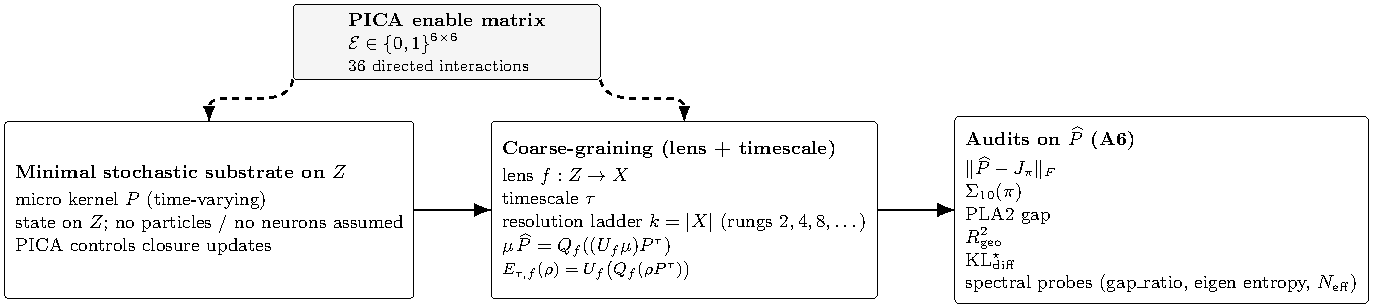
\includegraphics[width=0.92\linewidth]{fig/F1_pipeline.pdf}
\caption{Pipeline overview from micro substrate to audited macro dynamics, showing the canonical objects $\Z$, $f:\Z\to\X$, $\tau$, $\Phat$, $\Etauf$, and PICA enable matrix $\Epica$.}
\label{fig:F1_pipeline}
\end{figure}

\subsection{Minimal stochastic substrate and closure mechanisms}
\label{sec:methods:substrate}
A run is a stochastic process on an augmented state that includes at least the current effective micro kernel $P_t$ together with auxiliary variables used by the closure mechanisms (e.g., candidate lenses and packagings, route-mismatch scores, active timescale $\tau$, and accounting/budget state).
We denote the augmented state abstractly by $S_t$ and write the autonomous update as
\begin{equation}
S_{t+1} \sim \mathcal{U}_{\Epica}(S_t;\,\xi_t),
\end{equation}
where $\xi_t$ is the internal randomness and $\Epica$ is the enable matrix defined below.
The output of a run is an audit snapshot containing the effective kernel $P$ at the sampled step together with derived audit records.

\subsection{PICA: the six-primitive closure interaction algebra}
\label{sec:methods:pat}
Closure mechanisms are organized as six primitives \cite{Tsiokos2026SixBirds} with directed actor$\leftarrow$\hspace{0pt}informant interactions.
The interaction pattern is specified by the enable matrix
\begin{equation}
\Epica \in \{0,1\}^{6\times6},
\end{equation}
where $\Epica_{\alpha\beta}=1$ enables the interaction cell $P\alpha \leftarrow P\beta$.
Across all primitives there are $6\times6=36$ possible directed cells.
Each enabled cell is realized by a concrete operator acting on components of the augmented state (kernel rewriting, gating, protocol/timescale adaptation, lens selection, packaging/grouping, and accounting/budget feedback).
We treat PICA as an algebraic object: a \emph{subalgebra} is a subset of enabled cells subject to dependency closure constraints (e.g., consumers requiring their producers).
The full 36-cell catalog with statuses and short semantics is given in Table~\ref{tab:T1_PICA_cells}, and the ablation taxonomy used in this paper is summarized in Table~\ref{tab:T4A_taxonomy} and Table~\ref{tab:T4B_generators}.
The key experiment conditions (including baseline/full/generator families) are summarized in Table~\ref{tab:T2B_key_conditions}.
The 6$\times$6 interaction grid and key enable patterns are shown in Fig.~\ref{fig:F2_PICA_grid}.

\begin{figure}[htbp]
\centering
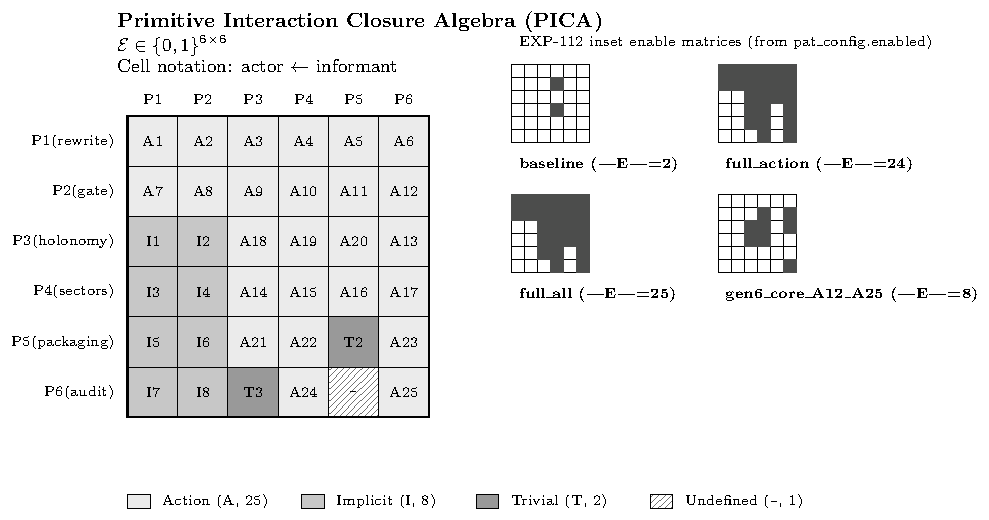
\includegraphics[width=0.92\linewidth]{fig/F2_PICA_grid.pdf}
\caption{PICA 6$\times$6 grid with class encoding aligned to Table~\ref{tab:T1_PICA_cells} statuses (Action/Implicit/Trivial/Undefined), plus EXP-112 inset enable matrices for baseline, full\_action, full\_all, and gen6\_core\_A12\_A25.}
\label{fig:F2_PICA_grid}
\end{figure}
% Auto-generated by paper/scripts/build_T1_PICA_cells.py
% Requires: \usepackage{booktabs,longtable}
\footnotesize
\setlength{\tabcolsep}{4pt}
\begin{longtable}{p{0.05\linewidth} p{0.12\linewidth} p{0.09\linewidth} p{0.19\linewidth} >{\raggedright\arraybackslash}p{0.35\linewidth}}
\caption{PICA 6$\times$6 cell catalog (A7.1): all actor$\leftarrow$informant positions with class, prerequisites, and one-line semantics.}\label{tab:T1_PICA_cells}\\
\toprule
Cell & Actor$\leftarrow$\newline Informant & Class & Prereqs & One-line semantics \\
\midrule
\endfirsthead
\toprule
Cell & Actor$\leftarrow$\newline Informant & Class & Prereqs & One-line semantics \\
\midrule
\endhead
\bottomrule
\endfoot
\bottomrule
\endlastfoot
A1 & P1\textless{}-P1 & Action & P1 rewrite history & History cooldown (avoid rewriting recently perturbed rows) \\
A2 & P1\textless{}-P2 & Action & row sparsity / gated-edge counts & Sparsity-guided row targeting \\
A3 & P1\textless{}-P3 & Action & route mismatch RM + active partition & RM-directed rewrite toward macro consistency \\
A4 & P1\textless{}-P4 & Action & active partition (selected P4 lens) & Sector-boundary targeting (near cluster boundaries) \\
A5 & P1\textless{}-P5 & Action & active packaging (selected P5) & Packaging defect targeting (idempotence failure) \\
A6 & P1\textless{}-P6 & Action & audit metrics / budget ledger & Budget-gated suppression of P1 when budget low \\
A7 & P2\textless{}-P1 & Action & P1 rewrite history & Protect rewrites (don't gate newly rewritten rows) \\
A8 & P2\textless{}-P2 & Action & P2 flip history / cooldown & Flip cooldown (don't re-flip recent edges) \\
A9 & P2\textless{}-P3 & Action & route mismatch RM + active partition & RM-guided gating (cross-cluster edges in high-RM clusters) \\
A10 & P2\textless{}-P4 & Action & active partition (selected P4 lens) & Spectral-guided gating (inter-cluster gating bias) \\
A11 & P2\textless{}-P5 & Action & active packaging (selected P5) & Package-boundary gating \\
A12 & P2\textless{}-P6 & Action & audit metrics / budget ledger & SBRC (repairs free; violations penalized) \\
I1 & P3\textless{}-P1 & Implicit & refresh cycle (implicit) & implicit (RM refresh after P1) \\
I2 & P3\textless{}-P2 & Implicit & refresh cycle (implicit) & implicit (RM refresh after P2) \\
A18 & P3\textless{}-P3 & Action & multi-scale RM convergence & adaptive tau from multi-scale RM convergence \\
A19 & P3\textless{}-P4 & Action & active partition + per-sector RM & per-sector mixing weights (high-RM sectors get more P1/P2) \\
A20 & P3\textless{}-P5 & Action & active packaging + per-package RM & packaging-derived mixing bias \\
A13 & P3\textless{}-P6 & Action & audit metrics / budget ledger & frob-modulated mixer (structure-driven explore/consolidate) \\
I3 & P4\textless{}-P1 & Implicit & refresh cycle (implicit) & implicit (partition refresh after P1) \\
I4 & P4\textless{}-P2 & Implicit & refresh cycle (implicit) & implicit (partition refresh after P2) \\
A14 & P4\textless{}-P3 & Action & route mismatch RM & RM-quantile partition \\
A15 & P4\textless{}-P4 & Action & active kernel spectrum & spectral partition (canonical lens) \\
A16 & P4\textless{}-P5 & Action & active packaging (selected P5) & package-derived partition \\
A17 & P4\textless{}-P6 & Action & audit metrics / EP flow & EP-flow partition \\
I5 & P5\textless{}-P1 & Implicit & refresh cycle (implicit) & implicit (packaging refresh after P1) \\
I6 & P5\textless{}-P2 & Implicit & refresh cycle (implicit) & implicit (packaging refresh after P2) \\
A21 & P5\textless{}-P3 & Action & route mismatch RM & RM-similarity packaging \\
A22 & P5\textless{}-P4 & Action & active partition (selected P4 lens) & sector-balanced packaging (split oversized clusters) \\
T2 & P5\textless{}-P5 & Trivial & tautology (trivial) & packaging idempotence (trivial) \\
A23 & P5\textless{}-P6 & Action & audit metrics / EP profile & EP-similarity packaging \\
I7 & P6\textless{}-P1 & Implicit & refresh cycle (implicit) & implicit (audit refresh after P1) \\
I8 & P6\textless{}-P2 & Implicit & refresh cycle (implicit) & implicit (audit refresh after P2) \\
T3 & P6\textless{}-P3 & Trivial & tautology (trivial) & trivial (RM is itself an audit metric; circular) \\
A24 & P6\textless{}-P4 & Action & active partition + per-sector EP & sector-specific budget rate multiplier from per-sector EP \\
U1 & P6\textless{}-P5 & Unde\-fined & undefined (circular) & undefined (no clear non-circular action) \\
A25 & P6\textless{}-P6 & Action & audit metrics / retention ledger & EP retention feedback cap (tighten when retention low) \\
\end{longtable}
% Auto-generated by paper/scripts/build_T4_taxonomy_generators.py
\begin{table*}[t]
\scriptsize
\centering
\caption{T4A: EXP-112 ablation taxonomy as algebraic cell-set constraints.}
\label{tab:T4A_taxonomy}
\resizebox{\textwidth}{!}{%
\begin{tabular}{l l p{5cm} r c p{4.5cm}}
\toprule
Family & Config labels & Algebraic definition & \#configs & $|S|$ range & Notes \\
\midrule
Null & `empty` & $S=\varnothing$ & 1 & 0-0 & No PICA cells enabled. \\
Baseline skeleton & `baseline` & $S=S_0=\{P2\leftarrow P4,\;P4\leftarrow P4\}$ & 1 & 2-2 & Minimal structural scaffold (A10+A15). \\
Full & `full\_action`, `full\_all` & $S_{\mathrm{full\_all}}$ = all Action cells (verified) ; $S_{\mathrm{full\_action}} = S_{\mathrm{full\_all}} \setminus \{A16\}$ & 2 & 24-25 & Observed $|S_{\mathrm{full\_action}}|$=24, $|S_{\mathrm{full\_all}}|$=25. \\
Generators & `gen*` & $S=\mathrm{cl}(S_0\cup G)$ where $G$ from gen-name tokens & 6 & 4-8 & Reusable low-cardinality generating subalgebras. \\
Leave-one-out & `loo\_*` & $S=S_{\mathrm{full\_action}}\setminus\{c\}$ & 22 & 23-23 & Single-cell removal tests around full\_action. \\
Full amputations & `fa\_no\_*` & $S=S_{\mathrm{full\_action}}\setminus D$ & 7 & 18-21 & Targeted amputations of full\_action components. \\
Actor-row subalgebras & `P*\_row`, `P*\_P*\_rows` & $S=\mathrm{cl}(S_0\cup\{c:\mathrm{actor}(c)\in R\})$ & 10 & 4-10 & Actor-focused slices of PICA. \\
Informant-column subalgebras & `col\_P*` & $S=\mathrm{cl}(S_0\cup\{c:\mathrm{informant}(c)=Pj\})$ & 6 & 4-8 & Informant-focused slices of PICA. \\
Singleton kernels & `A*\_only` & $S=\mathrm{cl}(S_0\cup\{A_i\})$ & 6 & 3-3 & One named action cell plus closure. \\
Pair kernels & `A*\_A*` (non-gen) & $S=\mathrm{cl}(S_0\cup\{A_i,A_j\})$ & 8 & 4-5 & Two named action cells plus closure. \\
\bottomrule
\end{tabular}}
\end{table*}

\begin{table*}[t]
\scriptsize
\centering
\caption{T4B: Generator subalgebras present in EXP-112 (config-level).}
\label{tab:T4B_generators}
\begin{tabular}{l r l l l}
\toprule
Generator config & $|S|$ & Named tokens & Extra closure cells & Enabled cells \\
\midrule
gen2\_A14\_A13 & 4 & A13; A14 & none & see CSV \\
gen3\_A13\_A14\_A19 & 5 & A13; A14; A19 & none & see CSV \\
gen3\_A13\_A18\_A19 & 5 & A13; A18; A19 & none & see CSV \\
gen4\_core & 6 & none & A13; A14; A18; A19 & see CSV \\
gen5\_core\_A25 & 7 & A25 & A13; A14; A18; A19 & see CSV \\
gen6\_core\_A12\_A25 & 8 & A12; A25 & A13; A14; A18; A19 & see CSV \\
\bottomrule
\end{tabular}
\end{table*}
% Auto-generated by paper/scripts/build_T2_tables.py
% Auto-generated by paper/scripts/build_T2_tables.py
\begin{table}[t]
\scriptsize
\centering
\caption{Key conditions used in the main narrative under the manifest-defined dataset union.}
\label{tab:T2B_key_conditions}
\begin{tabular}{l r l l r r r}
\toprule
Condition & $|E|$ & lens & packaging & $\tau_{\mathrm{cap}}$ & $\tau_{\mathrm{med}}$ & active$\tau$ rate \\
\midrule
Null (empty) & 0 & MinRM & MinRM & 10000 & 1.0 & 0.0000 \\
Baseline (baseline) & 2 & MinRM & MinRM & 10000 & 2.0 & 0.0000 \\
Full-Action (full\_action) & 24 & MinRM & MinRM & 10000 & 9.0 & 1.0000 \\
Full-All (full\_all) & 25 & MinRM & MinRM & 10000 & 8.0 & 1.0000 \\
Gen6-core (gen6\_core\_A12\_A25) & 8 & MinRM & MinRM & 10000 & 10.0 & 1.0000 \\
\bottomrule
\end{tabular}
\end{table}

\subsection{Coarse-graining and multiscale scan}
\label{sec:methods:coarse}
For auditing, we perform a multiscale scan that constructs macro kernels $\Phat(k)$ over a resolution ladder indexed by $k=|\X|$.
For each target scale $k_{\mathrm{target}}\in\{2,4,8,16,32,64\}$ (subject to $k_{\mathrm{target}}\le \min(64,\lfloor n/2\rfloor)$), we construct a partition $f_k:\Z\to\X$ using a spectral sign-pattern procedure:
we compute $d=\lceil \log_2(k_{\mathrm{target}})\rceil$ leading nontrivial eigenvectors of a reversible similarity transform of $P$, assign each micro state to a cluster by the sign pattern in $\{-,+\}^d$, and then compact away empty clusters to obtain an \emph{actual} cluster count $k=|\X|$.
Duplicate actual $k$ values are skipped so the scan yields a strictly increasing set of realized resolutions.

For each realized resolution $k$, we choose a timescale $\tau$ as follows.
If PICA provides an active $\tau$ (via enabled protocol/timescale mechanisms), we use that value; otherwise we use the default adaptive rule
\begin{equation}
\tau \;=\; \max\!\left(1,\left\lfloor \frac{\alpha}{g(P)}\right\rfloor\right),
\qquad
\tau \le 10^4,
\label{eq:tau-default}
\end{equation}
where $g(P)$ is the spectral gap proxy of $P$ and $\alpha$ is a fixed hyperparameter.
We then compute $P^\tau$ and construct the macro kernel $\Phat(k)=P^{\X}_{\tau,f_k}$ using \eqref{eq:macro-kernel}.

A central intermediate diagnostic used by lens/packaging selectors is \emph{route mismatch}, which quantifies within-cluster heterogeneity under $\tau$-step dynamics.
For a partition $f:\Z\to\X$ with $k=|\X|$, define for each $z\in\Z$ the projected $\tau$-step destination distribution over clusters:
\begin{equation}
p^{\X}_z(x') := \sum_{z'\in f^{-1}(x')} (P^\tau)_{zz'}.
\end{equation}
Let $\Phat(x,\cdot)$ be the induced macro row for cluster $x=f(z)$ (an average of $p^{\X}_z$ over the fiber).
The route mismatch score for cluster $x$ is the fiber-average $L^1$ deviation:
\begin{equation}
\mathrm{RM}(x) \;:=\; \frac{1}{|f^{-1}(x)|}\sum_{z\in f^{-1}(x)} \big\|p^{\X}_z - \Phat(x,\cdot)\big\|_1.
\label{eq:rm}
\end{equation}

\subsection{Audit metrics}
\label{sec:methods:audits}
All audits are computed on macro kernels $\Phat(k)$ for realized resolutions $k\le 64$.
Let $\pi$ be the stationary distribution of $\Phat$ (left eigenvector with $\pi^\top \Phat=\pi^\top$, normalized to sum to 1), and let $J_\pi:=\mathbf{1}\pi^\top$ be the rank-one kernel whose rows equal $\pi$.

\paragraph{Structure and mixing.}
We report the Frobenius distance from the rank-one stationary kernel:
\begin{equation}
\mathrm{frob}(\Phat) \;:=\; \|\Phat - J_\pi\|_F.
\label{eq:frob}
\end{equation}
We also report standard spectral diagnostics derived from the eigenvalues of a symmetrized operator (defined below): relaxation time $t_{\mathrm{rel}}=1/(1-|\lambda_2|)$, a gap ratio, an eigenvalue entropy over the nontrivial spectrum, and an effective spectral participation count.

\paragraph{Time-asymmetry and cyclic irreversibility.}
A stationary finite-horizon path-reversal asymmetry proxy is computed at horizon $T=10$:
\begin{equation}
\Sigma_{10}(\pi) \;:=\; 10 \sum_{i,j} \pi_i\,\Phat_{ij}\,\log\!\left(\frac{\Phat_{ij}}{\Phat_{ji}}\right),
\label{eq:sigma-pi}
\end{equation}
with numerical caps when $\Phat_{ij}>0$ but $\Phat_{ji}\approx 0$.
We additionally report a direct Frobenius antisymmetry score $\|\Phat-\Phat^\top\|_F$ and a 3-cycle chirality diagnostic.
For each directed triangle $(i,j,k)$ we define the cycle affinity
\begin{equation}
A(i,j,k) \;:=\; \log\!\left(\frac{\Phat_{ij}}{\Phat_{ji}}\right)+\log\!\left(\frac{\Phat_{jk}}{\Phat_{kj}}\right)+\log\!\left(\frac{\Phat_{ki}}{\Phat_{ik}}\right),
\end{equation}
again with numerical floors/caps.
We record the mean and maximum of $|A|$ across triangles and the count of triangles exceeding a fixed threshold.

At the run level we also compute a \emph{transient} finite-horizon entropy-production-like quantity $\sigma_u$ using a uniform initial macro distribution and including a boundary Shannon-entropy term.
Finally, we report $\sigma_{\mathrm{ratio}}$, defined (when well-conditioned) as the ratio of macro $\sigma_u$ to the corresponding micro value computed on $P^\tau$ at the matched $\tau$.

\paragraph{Lagrangian probes: least-action dominance and geometrizability.}
The Lagrangian probes treat per-edge negative log transition probability as an action surrogate:
\begin{equation}
\ell(i\to j) \;:=\; -\log\!\big(\max(\Phat_{ij},\varepsilon)\big),
\qquad
\varepsilon=10^{-15}.
\label{eq:edge-action}
\end{equation}
The per-step transition entropy is
\begin{equation}
H_{\mathrm{step}}(\Phat) \;:=\; -\sum_i \pi_i \sum_j \Phat_{ij}\,\log\!\big(\max(\Phat_{ij},\varepsilon)\big).
\label{eq:step-entropy}
\end{equation}

Least-action dominance is quantified by the two-step PLA2 gap.
Let $(\Phat^2)_{ik}$ be the two-step transition probability and define the two-step action
\[a_2(i,k):=-\log\bigl(\max\bigl((\Phat^2)_{ik},\,\varepsilon\bigr)\bigr).\]
Define the best two-step path cost through a single intermediate state:
\begin{equation}
a^\star(i,k) \;:=\; \min_j \left[\ell(i\to j)+\ell(j\to k)\right].
\end{equation}
The PLA2 gap is the stationary-weighted expected nonnegative discrepancy:
\begin{equation}
\mathrm{PLA2}(\Phat) \;:=\; \sum_{i,k} \pi_i (\Phat^2)_{ik}\, \max\!\big(0,\,a^\star(i,k)-a_2(i,k)\big).
\label{eq:pla2}
\end{equation}

To test geometrizability and diffusion-like structure we compute a reversible spectral embedding of $\Phat$.
We first define the time-reversal kernel $\Phat^\star_{ij}:=\pi_j \Phat_{ji}/\pi_i$ and the symmetrized kernel $\Phat_{\mathrm{sym}}=(\Phat+\Phat^\star)/2$.
Let $D=\mathrm{diag}(\sqrt{\pi})$ and form the symmetric matrix $S:=D\,\Phat_{\mathrm{sym}}\,D^{-1}$, whose eigenpairs are computed numerically.
Using the top $m\le 3$ nontrivial eigenvectors $v^{(1)},\dots,v^{(m)}$ (skipping the stationary direction), we define embedding coordinates
$q^{(\ell)}_i := v^{(\ell)}_i / \sqrt{\pi_i}$ and $q_i:=(q^{(1)}_i,\dots,q^{(m)}_i)$.

Geometrizability is assessed by the weighted $R^2$ of a linear relationship between action and squared distance:
\begin{equation}
d^2(i,j) := \|q_j-q_i\|_2^2,
\qquad
\ell(i\to j) \approx c_0 + c_1 d^2(i,j),
\end{equation}
where the $R^2$ is computed over directed edges weighted by $\pi_i\Phat_{ij}$.
We report this as $R^2_{\mathrm{geo}}$.

Finally, we fit a minimal diffusion-kernel model of the form
\begin{equation}
\widehat{\Phat}_{ij}(\alpha) \;\propto\; \exp\!\big(-\alpha\, d^2(i,j)\big),
\end{equation}
row-normalized for each $i$.
We choose $\alpha^\star$ to minimize the stationary-weighted rowwise KL divergence
\begin{equation}
\mathrm{KL}_{\mathrm{diff}}^\star \;:=\; \min_{\alpha>0}\sum_i \pi_i\, D_{\mathrm{KL}}\!\left(\Phat(i,\cdot)\,\|\,\widehat{\Phat}(i,\cdot;\alpha)\right),
\label{eq:diff-kl}
\end{equation}
and report both $\alpha^\star$ and $\mathrm{KL}_{\mathrm{diff}}^\star$.
These quantities are undefined (reported as missing) when the embedding cannot be constructed reliably (e.g., degenerate stationary mass or too small $k$).

\subsection{Experiment design and analysis protocol}
\label{sec:methods:analysis}
We evaluate a manifest-defined campaign\_v3 union across four substrate sizes $n\in\{32,64,128,256\}$: an exhaustive EXP-112 suite for $n\le 128$ plus a selected scaling suite at $n=256$ that combines controls (EXP-F1/\allowbreak{}EXP-107) with targeted EXP-112 configurations probing partition competition, generator cores, row removals, and a small leave-one-out subset, totaling 2307 runs (Tables~\ref{tab:T2A_dataset_overview}--\ref{tab:T2C_n256_suites}).
The EXP-112 selective $n=256$ subset has incomplete seeds due to 26 truncated wave\_2 logs; all analyses explicitly report seed support and apply the preregistered min-support filter.
% Auto-generated by paper/scripts/build_T2_tables.py
% Auto-generated by paper/scripts/build_T2_tables.py
\begin{table}[t]
\scriptsize
\centering
\caption{Paper dataset overview by micro size (manifest-defined union).}
\label{tab:T2A_dataset_overview}
\resizebox{\linewidth}{!}{%
\begin{tabular}{lrrrrl l rrrr}
\toprule
$n$ & Runs & Configs & Seeds/config & Exp IDs & $\tau_{\mathrm{med}}$ & $\tau_{\min}$ & $\tau_{\max}$ & active$\tau$ rate & REV count & REV rate \\
\midrule
32 & 690 & 69 & 10/10/10 & EXP-112 & 37.5 & 1.0 & 10000.0 & 0.5652 & 6 & 0.0087 \\
64 & 690 & 69 & 10/10/10 & EXP-112 & 11.0 & 1.0 & 1989.0 & 0.5652 & 0 & 0.0000 \\
128 & 690 & 69 & 10/10/10 & EXP-112 & 2.0 & 1.0 & 970.0 & 0.5652 & 0 & 0.0000 \\
256 & 237 & 26 & 5/10/10 & EXP-107,EXP-112,EXP-F1 & 1.0 & 1.0 & 4.0 & 0.4262 & 0 & 0.0000 \\
ALL & 2307 & 79 & 5/10/10 & EXP-107,EXP-112,EXP-F1 & 5.0 & 1.0 & 10000.0 & 0.5509 & 6 & 0.0026 \\
\bottomrule
\end{tabular}}
\end{table}
% Auto-generated by paper/scripts/build_T2_tables.py
\begin{table}[t]
\scriptsize
\centering
\caption{Wave\_2 ($n=256$) experiment suites: expected jobs, extracted audits, and paper-use status.}
\label{tab:T2C_n256_suites}
\resizebox{\linewidth}{!}{%
\begin{tabular}{l r r r l c p{5cm}}
\toprule
Exp ID & Configs & Jobs expected & Audits extracted & Seeds & Used in paper & Notes \\
\midrule
EXP-F1 & 1 & 10 & 10 & 0-9 & yes &  \\
EXP-100 & 13 & 130 & 130 & 0-9 & no &  \\
EXP-101 & 7 & 70 & 70 & 0-9 & no &  \\
EXP-106 & 13 & 130 & 130 & 0-9 & no &  \\
EXP-107 & 13 & 130 & 130 & 0-9 & yes &  \\
EXP-109 & 1 & 10 & 10 & 0-9 & no &  \\
EXP-110 & 1 & 10 & 10 & 0-9 & no &  \\
EXP-112 & 15 & 150 & 124 & 0-9 & yes & 26 truncated logs overall;\allowbreak{} EXP-112 extracted=124/150 \\
\bottomrule
\end{tabular}}
\end{table}
The n=256 wave\_2 experiment suites are summarized in Table~\ref{tab:T2C_n256_suites}.

Key condition families (null/\allowbreak{}baseline/\allowbreak{}full/\allowbreak{}generators/\allowbreak{}leave-one-out and others) are defined algebraically in Table~\ref{tab:T4A_taxonomy}.

For scan curves, we aggregate audit metrics across seeds at fixed $(\text{config},n,k)$.
To avoid low-support artifacts, a scan point is plotted only if at least 5 seeds are present at that rung (min-support filter).
For run-level headline summaries we define, for each run and metric $m(k)$, the \emph{core-rung median} over $k\ge 4$:
\begin{equation}
\tilde m \;:=\; \mathrm{median}\{m(k): k\ge 4\},
\end{equation}
yielding the headline metrics reported in Table~\ref{tab:T3_headline_metrics}.

Uncertainty intervals are computed by deterministic bootstrapping of the median (5000 resamples with a fixed RNG seed), and effect sizes are reported using a robust MAD-standardized difference:
\begin{equation}
ES_{\mathrm{MAD}}(x,y)=\frac{\mathrm{median}(x)-\mathrm{median}(y)}{\tfrac12(\mathrm{MAD}(x)+\mathrm{MAD}(y))+\varepsilon},
\qquad \varepsilon=10^{-15}.
\end{equation}
Correlations among Lagrange probes are assessed at an anchor rung $k=4$ using Spearman rank correlation with Benjamini--Hochberg FDR correction within each $n$ (Table~\ref{tab:T5A_correlations}).
A fixed regression tests diffusion misfit $\mathrm{KL}_{\mathrm{diff}}^\star(k{=}4)$ against a predefined partition-competition subset, with bootstrap confidence intervals (Table~\ref{tab:T5B_regression}).

Runs that fall into an effectively reversible regime are tracked separately.
Operationally, a run is labeled REV if its macro-level asymmetry and cycle-chirality diagnostics are numerically negligible (near-zero $\Sigma_{10}(\pi)$ and cycle scores with zero detected chiral triangles), and REV prevalence is summarized as part of the robustness checklist (Table~\ref{tab:T6_robustness}).
% Auto-generated by paper/scripts/build_T6_robustness.py
% Auto-generated by paper/scripts/build_T6_robustness.py
% Auto-generated by paper/scripts/build_T6_robustness.py
\begin{landscape}
\scriptsize
\setlength{\tabcolsep}{2pt}
\begin{longtable}{>{\raggedright\arraybackslash}p{0.14\linewidth} c >{\raggedright\arraybackslash}p{0.34\linewidth} >{\raggedright\arraybackslash}p{0.14\linewidth} >{\raggedright\arraybackslash}p{0.22\linewidth}}
\caption{Robustness checklist (pre-registered-like; A10). Outcomes are auto-filled from deposited artifacts where computable; pending items are explicitly marked.}
\label{tab:T6_robustness} \\
\toprule
Check & Status & Auto-filled summary & Evidence & Notes \\
\midrule
\endfirsthead
\multicolumn{5}{c}{\tablename\ \thetable{} -- continued} \\
\toprule
Check & Status & Auto-filled summary & Evidence & Notes \\
\midrule
\endhead
\bottomrule
\endfoot
R1 Coverage completeness & PASS & [yes] runs=2307/2307;\allowbreak  per\_n=32:690,64:690,128:690,256:237;\allowbreak  cfg\_per\_n=32:69,64:69,128:69,256:26 & run\_summary\_table;\allowbreak T2\_QA & Exact coverage required. \\
R2 Seed support per (config,n) & PARTIAL & [yes] seeds\_per\_(config,n)=5/10/10 & run\_summary\_table;\allowbreak T2\_QA & n\textless{}=128 expected 10/10/10;\allowbreak  n=256 selective suite allows partial seeds. \\
R3 PICA config consistency across runs & PASS & [yes] pat\_config\_consistency\_all\_configs=True & T2\_QA & Configuration drift would invalidate condition-level claims. \\
R4 Scan min-support enforcement & PARTIAL & [yes] n32:baseline=[16];\allowbreak  n32:full\_action=[16];\allowbreak  n32:full\_all=[16];\allowbreak  n64:baseline=[32];\allowbreak  n64:full\_action=[32];\allowbreak  n64:full\_all=[32];\allowbreak  n128:baseline=[2, 64];\allowbreak  n128:full\_action=[2, 64];\allowbreak  n128:full\_all=[2, 64];\allowbreak  n256:baseline=[2];\allowbreak  n256:full\_action=[2, 64];\allowbreak  n256:full\_all=[2, 64] & F3\_QA;\allowbreak F4\_QA & Mid/low rung drops observed;\allowbreak  interpret affected curves cautiously. \\
R5 Lagrange-probe missingness (n=128) & PASS & [yes] geo=0.204;\allowbreak  diff\_kl=0.204;\allowbreak  overall=0.204 & F4\_QA & PASS threshold: overall missingness \textless{} 0.25. \\
R6 Tau policy outcomes & PASS & [yes] tau\_ranges=\allowbreak n32[1,1830],\allowbreak n64[1,632],\allowbreak n128[1,970],\allowbreak n256[1,4];\allowbreak  rates\_reported=True & F7\_tau\_stats;\allowbreak F7\_QA & Differences across configs are expected;\allowbreak  reporting completeness is required. \\
R7 Tau overlap feasibility & FAIL & [yes] n32:overlap=0,jacc=0.000;\allowbreak  n64:overlap=0,jacc=0.000;\allowbreak  n128:overlap=1,jacc=0.143;\allowbreak  n256:overlap=0,jacc=0.000 & run\_summary\_table & FAIL implies direct tau-controlled comparisons are not feasible without additional matching. \\
R8 REV prevalence and handling & PASS & [yes] n32:6/690 (0.0087);\allowbreak  n64:0/690 (0.0000);\allowbreak  n128:0/690 (0.0000);\allowbreak  n256:0/237 (0.0000) & run\_summary\_table;\allowbreak F8\_REV\_stats & REV is explicitly quantified and excluded where required (e.g., T5). \\
R9 sigma\_ratio missingness & PASS & [yes] n32:empty=0.00;\allowbreak  n32:baseline=0.20;\allowbreak  n32:full\_action=1.00;\allowbreak  n32:full\_all=0.80;\allowbreak  n64:empty=0.00;\allowbreak  n64:baseline=0.10;\allowbreak  n64:full\_action=0.90;\allowbreak  n64:full\_all=0.80;\allowbreak  n128:empty=0.00;\allowbreak  n128:baseline=0.00;\allowbreak  n128:full\_action=0.00;\allowbreak  n128:full\_all=0.20;\allowbreak  n256:empty=0.00;\allowbreak  n256:baseline=0.00;\allowbreak  n256:full\_action=0.00;\allowbreak  n256:full\_all=0.00 & F8\_QA;\allowbreak F8\_sigma\_stats & PASS threshold uses n=128 full\_action/full\_all missingness \textless{}= 0.2. \\
R10 LOO integrity & PASS & [yes] valid\_single\_removal=22/22 & F6\_QA;\allowbreak loo\_cell\_map & Expected 22/22 for strict LOO interpretation. \\
R11 Headline metric effective N & PARTIAL & [yes] n32:full\_all=5;\allowbreak  n64:full\_all=7;\allowbreak  n256:gen6\_core\_A12\_A25=0 & T3\_QA & PARTIAL indicates reduced effective sample size for some config/n blocks. \\
R12 Anchor-rung k=4 probe coverage & PASS & [yes] n32:543-684;\allowbreak  n64:649-690;\allowbreak  n128:689-690;\allowbreak  n256:237-237 & T5\_QA & Thresholds: n32\textgreater{}=500, n64\textgreater{}=640, n128\textgreater{}=680, n256\textgreater{}=200 for N\_pair\_min. \\
\end{longtable}
\end{landscape}



\section{Results}
\label{sec:results}

All results reported below come from a manifest-defined campaign\_v3 union across four micro sizes $n\in\{32,64,128,256\}$ (Table~\ref{tab:T2A_dataset_overview}).
For $n\le 128$ we use the exhaustive EXP-112 suite comprising 69 PICA subalgebras with ten seeds per $(\mathrm{config},n)$ (2070 runs total), while $n=256$ is evaluated via a selected scaling suite that combines controls (empty/baseline/full\_action/full\_all) with targeted EXP-112 configurations (Table~\ref{tab:T2C_n256_suites}), yielding 237 $n=256$ runs in the manifest union.
Unless stated otherwise, scan curves aggregate across seeds at fixed $(\mathrm{config},n,k)$ with the preregistered min-support filter (at least 5 seeds per rung), and run-level headline metrics use the core-rung median over $k\ge 4$ (Methods).

\subsection{C1: Full PICA activation reshapes multiscale structure and suppresses macro time-asymmetry}
Figure~\ref{fig:F3_multiscale} shows how (i) structural distance from stationarity and (ii) macro time-asymmetry vary with coarse-graining resolution $k$.
Across sizes, the baseline skeleton and the null substrate exhibit strong scale dependence: increasing resolution generally increases both structural separation and time-asymmetry.
In contrast, activating the full Action set (Full-Action / Full-All) produces a qualitatively different regime in which macro time-asymmetry $\Sigma_{10}(\pi)$ is strongly suppressed across rungs and sizes (Table~\ref{tab:T3_headline_metrics}).

\begin{figure}[htbp]
\centering
\textbf{Structure: $\mathrm{frob}(\Phat)$ vs. $k$.}\par\medskip
\begin{tabular}{@{}cc@{}}
  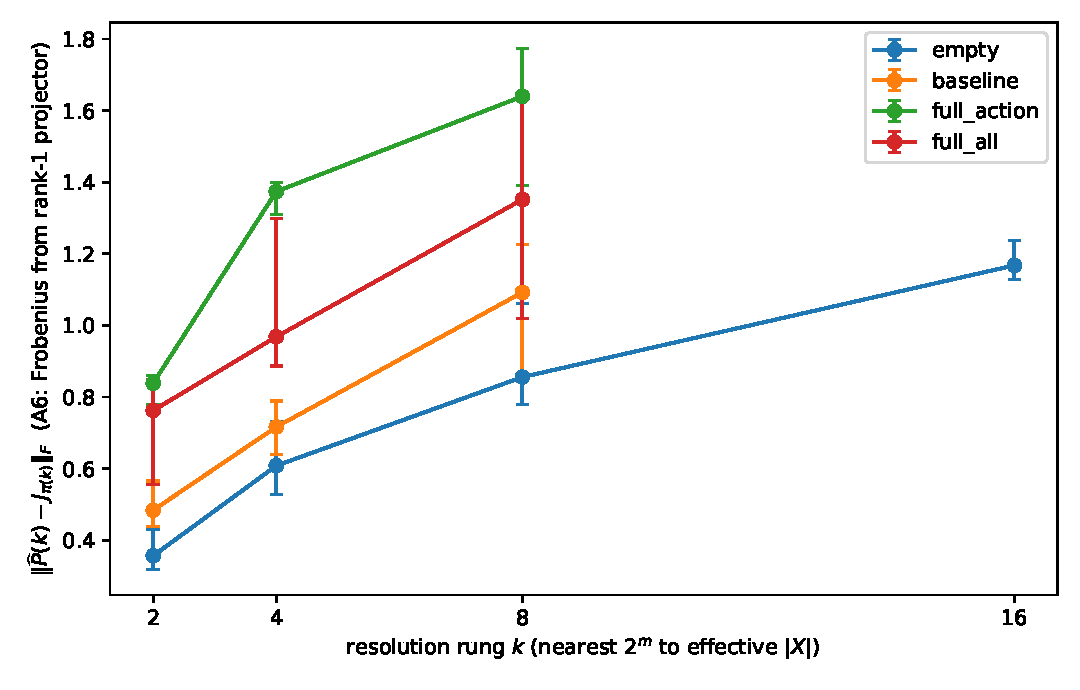
\includegraphics[width=0.49\linewidth]{fig/F3a_n32.pdf} &
  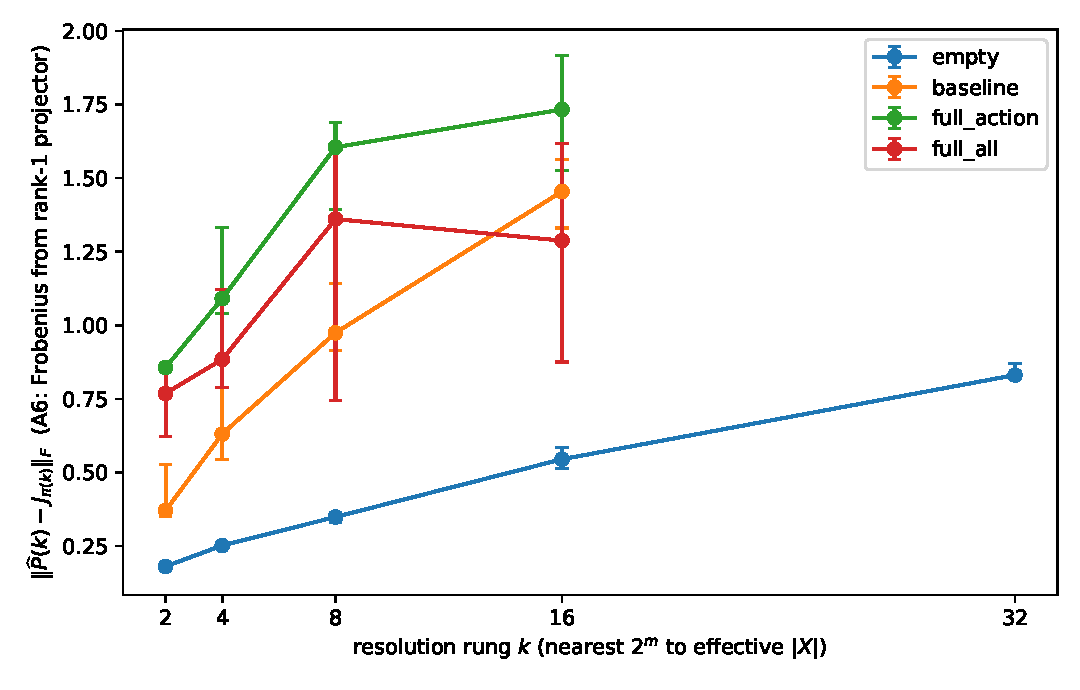
\includegraphics[width=0.49\linewidth]{fig/F3a_n64.pdf}\\[0.3em]
  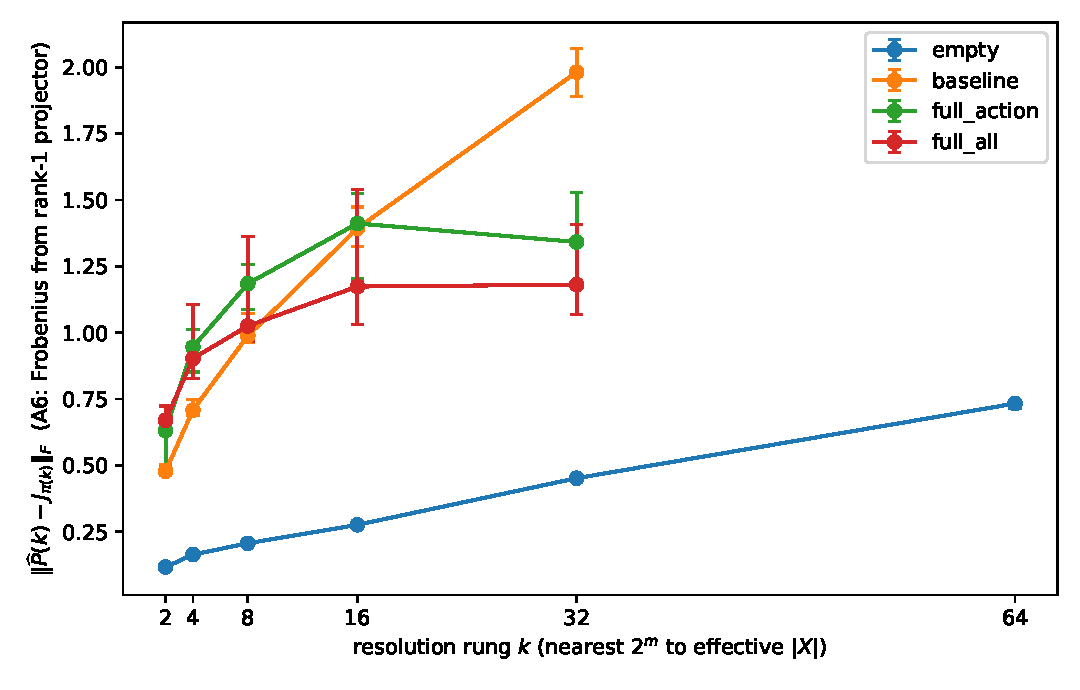
\includegraphics[width=0.49\linewidth]{fig/F3a_n128.pdf} &
  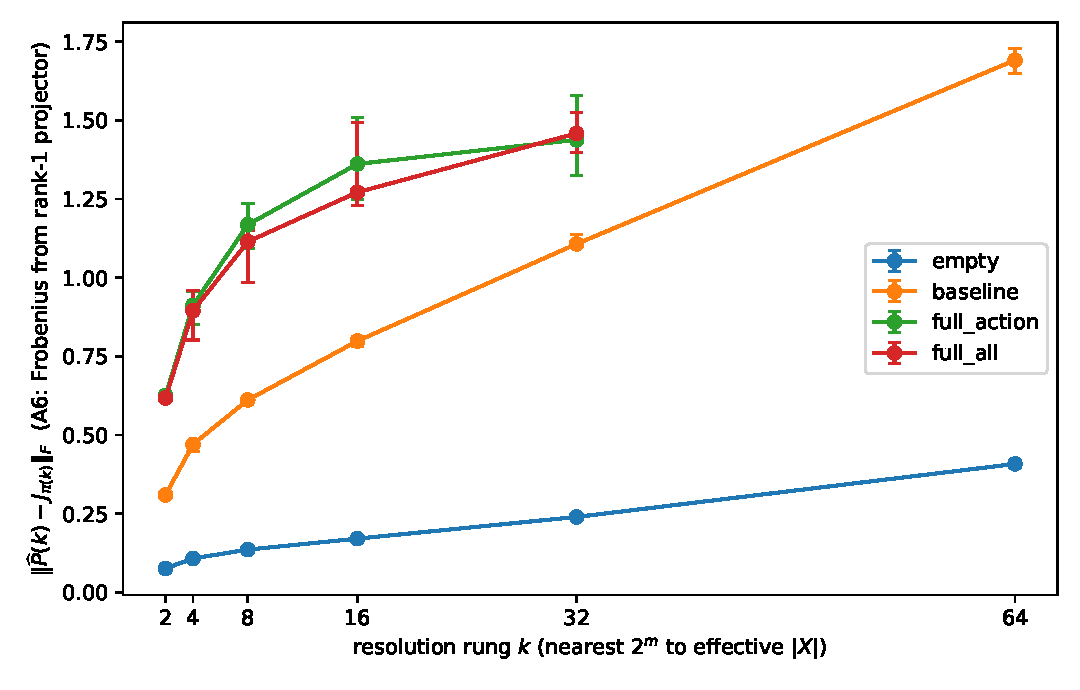
\includegraphics[width=0.49\linewidth]{fig/F3a_n256.pdf}\\
\end{tabular}
\par\medskip
\textbf{Arrow-of-time: $\log_{10}(1+\Sigma_{10}(\pi(k)))$ vs. $k$.}\par\medskip
\begin{tabular}{@{}cc@{}}
  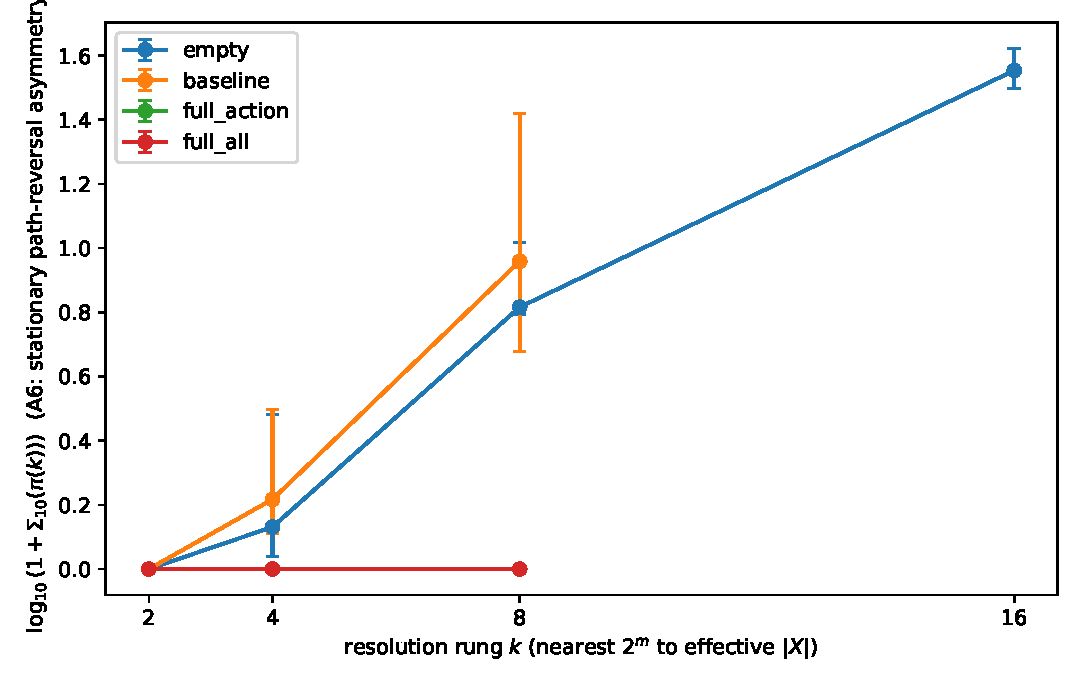
\includegraphics[width=0.49\linewidth]{fig/F3b_n32.pdf} &
  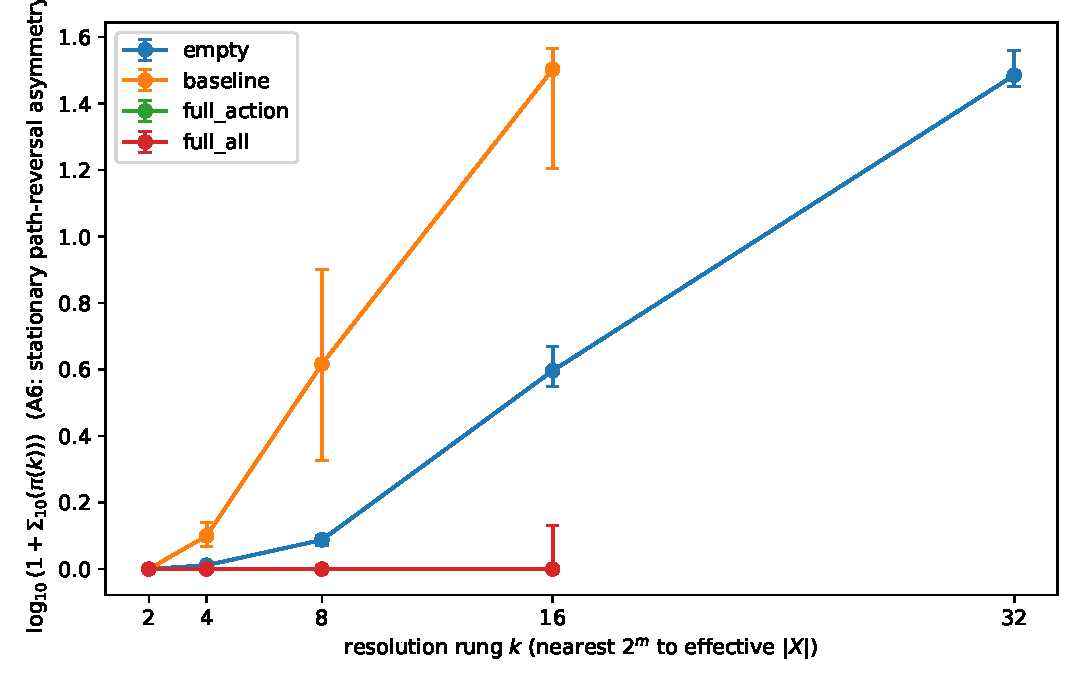
\includegraphics[width=0.49\linewidth]{fig/F3b_n64.pdf}\\[0.3em]
  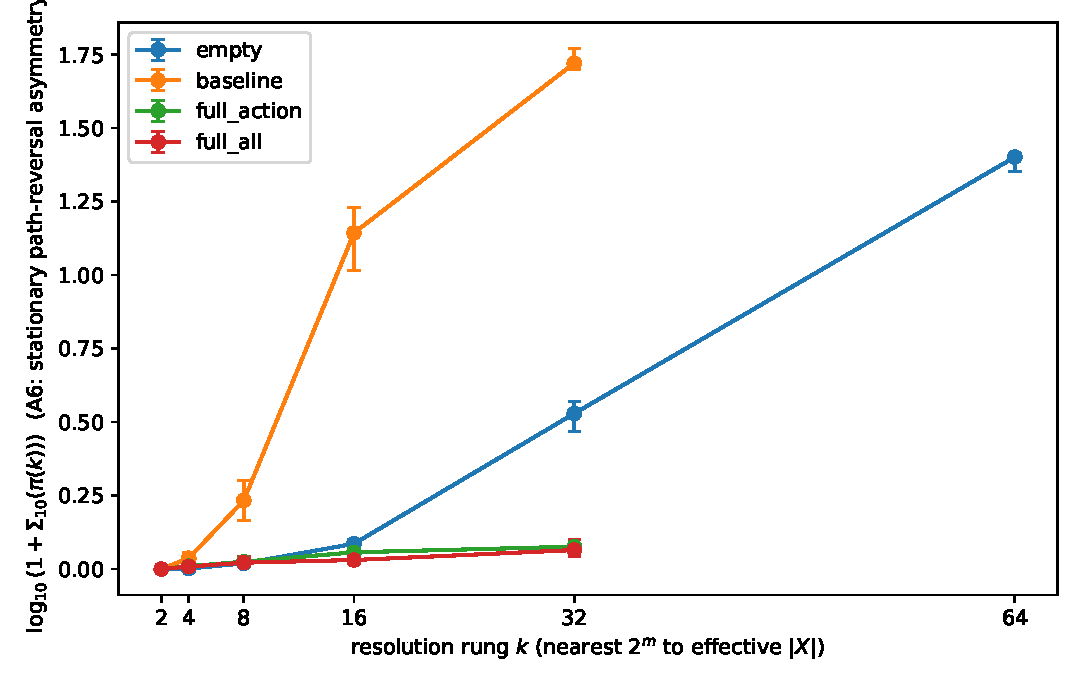
\includegraphics[width=0.49\linewidth]{fig/F3b_n128.pdf} &
  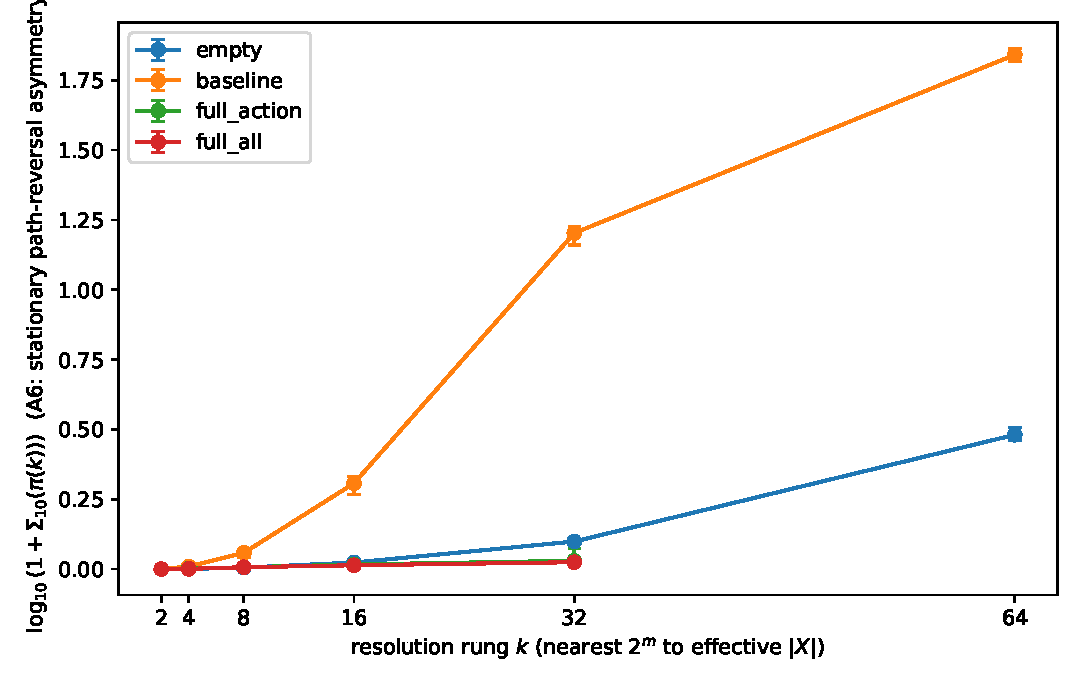
\includegraphics[width=0.49\linewidth]{fig/F3b_n256.pdf}\\
\end{tabular}
\caption{F3: Multiscale scan curves for structure and time-asymmetry across $n\in\{32,64,128,256\}$. Curves report seed medians with interquartile ranges; only scan rungs with at least 5 seeds are plotted. Conditions shown: Null (empty), Baseline (baseline), Full-Action (full\_action), and Full-All (full\_all). The x-axis uses resolution rung $k$ defined as the nearest power-of-two to effective $k_{\mathrm{eff}}=|\X|$. The arrow-of-time panels plot $\log_{10}(1+\Sigma_{10}(\pi(k)))$.}
\label{fig:F3_multiscale}
\end{figure}

\begin{landscape}
\scriptsize
\setlength{\tabcolsep}{2pt}
% Auto-generated by paper/scripts/build_T3_headline_metrics.py
% Auto-generated by paper/scripts/build_T3_headline_metrics.py
\begin{longtable}{l r >{\raggedright\arraybackslash}p{0.142\linewidth} >{\raggedright\arraybackslash}p{0.142\linewidth} >{\raggedright\arraybackslash}p{0.142\linewidth} >{\raggedright\arraybackslash}p{0.142\linewidth} >{\raggedright\arraybackslash}p{0.142\linewidth}}
\caption{Headline metrics by condition and micro size, using medians over core rungs ($k\geq 4$). Entries report median with bootstrap 95\% CI ($B=5000$), plus $\Delta$ vs baseline and robust $ES_{\mathrm{MAD}}$. NA indicates the condition is not present in the n=256 selective suite.}
\label{tab:T3_headline_metrics} \\
\toprule
Condition & $|E|$ & $\widetilde{\mathrm{frob}}$ & $\widetilde{\Sigma}_{10}(\pi)$ & $\widetilde{R^2_{\mathrm{geo}}}$ & $\widetilde{\mathrm{PLA2}}$ & $\widetilde{\mathrm{KL}^{\star}_{\mathrm{diff}}}$ \\
\midrule
\endfirsthead
\multicolumn{7}{c}{\tablename\ \thetable{} -- continued} \\
\toprule
Condition & $|E|$ & $\widetilde{\mathrm{frob}}$ & $\widetilde{\Sigma}_{10}(\pi)$ & $\widetilde{R^2_{\mathrm{geo}}}$ & $\widetilde{\mathrm{PLA2}}$ & $\widetilde{\mathrm{KL}^{\star}_{\mathrm{diff}}}$ \\
\midrule
\endhead
\bottomrule
\endfoot
\midrule
\multicolumn{7}{l}{\textbf{$n=32$}} \\
Null (empty) & 0 & 0.856 [0.772, 1.1] \newline {\scriptsize $\Delta$ -0.112 [-0.421, 0.248]; ES -0.861} & 5.54 [5.05, 11.7] \newline {\scriptsize $\Delta$ -0.547 [-24.9, 10.4]; ES -0.241} & 0.125 [0.0915, 0.178] \newline {\scriptsize $\Delta$ 0.000765 [-0.0747, 0.0742]; ES 0.0348} & 0.795 [0.695, 0.883] \newline {\scriptsize $\Delta$ 0.189 [0.113, 0.41]; ES 2.44} & 0.236 [0.183, 0.272] \newline {\scriptsize $\Delta$ -0.0682 [-0.112, 0.0491]; ES 0.0268} \\
Baseline (baseline) & 2 & 0.989 [0.798, 1.23] \newline {\scriptsize baseline} & 6.17 [2.85, 26.9] \newline {\scriptsize baseline} & 0.123 [0.0454, 0.196] \newline {\scriptsize baseline} & 0.555 [0.381, 0.684] \newline {\scriptsize baseline} & 0.236 [0.221, 0.318] \newline {\scriptsize baseline} \\
Full-Action (full\_action) & 24 & 1.49 [1.25, 1.57] \newline {\scriptsize $\Delta$ 0.454 [0.128, 0.738]; ES 2.98} & 6.66e-11 [6.1e-11, 8.41e-11] \newline {\scriptsize $\Delta$ -6.17 [-26.9, -2.85]; ES -2.92} & 0.177 [0.139, 0.22] \newline {\scriptsize $\Delta$ 0.087 [-0.0833, 0.152]; ES 1.11} & 0.0258 [4.04e-13, 0.127] \newline {\scriptsize $\Delta$ -0.42 [-0.655, -0.37]; ES -6.72} & 1.71e-11 [1.35e-11, 0.0684] \newline {\scriptsize $\Delta$ -0.226 [-0.28, -0.197]; ES -22.1} \\
Full-All (full\_all) & 25 & 1.08 [0.93, 1.57] \newline {\scriptsize $\Delta$ 0.16 [-0.168, 0.636]; ES 0.378} & 8.03e-11 [6.17e-11, 1.49] \newline {\scriptsize $\Delta$ -3.76 [-26.9, -0.163]; ES -2.92} & 1.59e-10 [4.6e-12, 0.114] \newline {\scriptsize $\Delta$ -0.0782 [-0.244, 0.0682]; ES -4.01} & 0.27 [0.056, 0.491] \newline {\scriptsize $\Delta$ -0.474 [-0.51, 0.185]; ES -1.64} & 0.0308 [0.0252, 0.368] \newline {\scriptsize $\Delta$ -0.197 [-0.317, 0.0191]; ES -15.2} \\
Gen6-core (gen6\_core\_A12\_A25) & 8 & 1.01 [0.829, 1.16] \newline {\scriptsize $\Delta$ -0.0213 [-0.18, 0.386]; ES 0.135} & 4.25e-09 [7.35e-11, 0.35] \newline {\scriptsize $\Delta$ -6.17 [-26.8, -2.28]; ES -2.92} & 1.54e-09 [1.28e-12, 0.188] \newline {\scriptsize $\Delta$ -0.0966 [-0.244, 0.0892]; ES -4.01} & 0.454 [0.181, 0.756] \newline {\scriptsize $\Delta$ -0.142 [-0.397, 0.262]; ES -0.523} & 0.151 [0.0477, 0.327] \newline {\scriptsize $\Delta$ -0.16 [-0.243, 0.0632]; ES -1.2} \\
\midrule
\multicolumn{7}{l}{\textbf{$n=64$}} \\
Null (empty) & 0 & 0.455 [0.423, 0.477] \newline {\scriptsize $\Delta$ -0.707 [-0.783, -0.514]; ES -10.1} & 1.59 [1.33, 2.16] \newline {\scriptsize $\Delta$ -5.81 [-11.5, -0.0308]; ES -2.17} & 0.104 [0.0734, 0.165] \newline {\scriptsize $\Delta$ -0.0463 [-0.0611, 0.082]; ES -0.472} & 1.5 [1.45, 1.55] \newline {\scriptsize $\Delta$ 0.751 [0.668, 0.875]; ES 13.5} & 0.115 [0.0861, 0.135] \newline {\scriptsize $\Delta$ -0.0855 [-0.178, -0.00947]; ES -2.37} \\
Baseline (baseline) & 2 & 1.14 [0.974, 1.24] \newline {\scriptsize baseline} & 7.4 [1.96, 13.4] \newline {\scriptsize baseline} & 0.126 [0.0436, 0.166] \newline {\scriptsize baseline} & 0.788 [0.615, 0.832] \newline {\scriptsize baseline} & 0.21 [0.105, 0.312] \newline {\scriptsize baseline} \\
Full-Action (full\_action) & 24 & 1.5 [1.27, 1.65] \newline {\scriptsize $\Delta$ 0.444 [0.13, 0.595]; ES 2.64} & 6.72e-11 [6.2e-11, 7.92e-11] \newline {\scriptsize $\Delta$ -7.31 [-13.4, -1.96]; ES -2.93} & 0.00647 [9.36e-14, 0.223] \newline {\scriptsize $\Delta$ -0.061 [-0.177, 0.212]; ES -4.17} & 0.0563 [3.26e-13, 0.278] \newline {\scriptsize $\Delta$ -0.617 [-0.802, -0.494]; ES -12.7} & 0.115 [1.29e-11, 0.381] \newline {\scriptsize $\Delta$ -0.131 [-0.268, 0.173]; ES -1.08} \\
Full-All (full\_all) & 25 & 1.26 [0.707, 1.43] \newline {\scriptsize $\Delta$ 0.00757 [-0.436, 0.448]; ES 0.539} & 7.23e-11 [6.85e-11, 0.164] \newline {\scriptsize $\Delta$ -7.18 [-13.2, -1.96]; ES -2.93} & 0.152 [6.72e-13, 0.292] \newline {\scriptsize $\Delta$ -0.0245 [-0.164, 0.231]; ES 0.264} & 0.433 [4.66e-13, 0.854] \newline {\scriptsize $\Delta$ -0.179 [-0.762, 0.105]; ES -1.5} & 0.216 [1.65e-11, 0.265] \newline {\scriptsize $\Delta$ -0.021 [-0.169, 0.167]; ES 0.121} \\
Gen6-core (gen6\_core\_A12\_A25) & 8 & 1.01 [0.789, 1.59] \newline {\scriptsize $\Delta$ -0.0877 [-0.349, 0.518]; ES -0.755} & 0.0538 [7.03e-11, 1.63] \newline {\scriptsize $\Delta$ -7.4 [-13.1, -1.23]; ES -2.88} & 0.0317 [3.71e-12, 0.104] \newline {\scriptsize $\Delta$ -0.0666 [-0.156, 0.092]; ES -2.28} & 0.704 [0.313, 0.974] \newline {\scriptsize $\Delta$ -0.107 [-0.569, 0.212]; ES -0.492} & 0.268 [0.11, 0.302] \newline {\scriptsize $\Delta$ 0.0781 [-0.212, 0.261]; ES 1.24} \\
\midrule
\multicolumn{7}{l}{\textbf{$n=128$}} \\
Null (empty) & 0 & 0.276 [0.271, 0.289] \newline {\scriptsize $\Delta$ -1.04 [-1.11, -0.864]; ES -25.6} & 0.219 [0.202, 0.26] \newline {\scriptsize $\Delta$ -10 [-13.7, -4.35]; ES -4.54} & 0.135 [0.0817, 0.174] \newline {\scriptsize $\Delta$ 0.00527 [-0.0325, 0.0875]; ES 1.35} & 2.03 [1.98, 2.08] \newline {\scriptsize $\Delta$ 1.25 [1.18, 1.3]; ES 38} & 0.0518 [0.0431, 0.0761] \newline {\scriptsize $\Delta$ -0.343 [-0.379, -0.252]; ES -10.8} \\
Baseline (baseline) & 2 & 1.32 [1.14, 1.38] \newline {\scriptsize baseline} & 10.3 [4.57, 14] \newline {\scriptsize baseline} & 0.0915 [0.0786, 0.137] \newline {\scriptsize baseline} & 0.795 [0.735, 0.818] \newline {\scriptsize baseline} & 0.386 [0.327, 0.429] \newline {\scriptsize baseline} \\
Full-Action (full\_action) & 24 & 1.25 [1.07, 1.3] \newline {\scriptsize $\Delta$ -0.0939 [-0.269, 0.223]; ES -0.933} & 0.0778 [0.0483, 0.146] \newline {\scriptsize $\Delta$ -10.2 [-13.7, -4.52]; ES -4.59} & 0.124 [0.037, 0.328] \newline {\scriptsize $\Delta$ 0.0274 [-0.0832, 0.232]; ES 0.597} & 0.571 [0.459, 0.854] \newline {\scriptsize $\Delta$ -0.233 [-0.283, 0.0533]; ES -2.84} & 0.572 [0.395, 0.655] \newline {\scriptsize $\Delta$ 0.194 [-0.041, 0.309]; ES 3.41} \\
Full-All (full\_all) & 25 & 1.07 [0.961, 1.46] \newline {\scriptsize $\Delta$ -0.176 [-0.383, 0.416]; ES -2.42} & 0.0628 [0.0221, 0.165] \newline {\scriptsize $\Delta$ -9.73 [-13.9, -4.52]; ES -4.59} & 0.115 [0.0561, 0.157] \newline {\scriptsize $\Delta$ 0.0114 [-0.0672, 0.0681]; ES 0.771} & 0.45 [0.327, 0.725] \newline {\scriptsize $\Delta$ -0.292 [-0.469, -0.0865]; ES -3.56} & 0.642 [0.311, 0.789] \newline {\scriptsize $\Delta$ 0.303 [-0.122, 0.402]; ES 2} \\
Gen6-core (gen6\_core\_A12\_A25) & 8 & 1.3 [1.03, 1.4] \newline {\scriptsize $\Delta$ 0.0545 [-0.14, 0.0974]; ES -0.197} & 2.22 [0.38, 5.85] \newline {\scriptsize $\Delta$ -5.66 [-10.3, -2.44]; ES -2.58} & 0.206 [0.138, 0.262] \newline {\scriptsize $\Delta$ 0.0779 [0.0386, 0.138]; ES 3.19} & 0.711 [0.584, 0.933] \newline {\scriptsize $\Delta$ -0.0307 [-0.217, 0.119]; ES -0.964} & 0.474 [0.392, 0.523] \newline {\scriptsize $\Delta$ 0.123 [0.00532, 0.162]; ES 1.86} \\
\midrule
\multicolumn{7}{l}{\textbf{$n=256$}} \\
Null (empty) & 0 & 0.171 [0.168, 0.174] \newline {\scriptsize $\Delta$ -0.626 [-0.646, -0.601]; ES -58} & 0.055 [0.0496, 0.064] \newline {\scriptsize $\Delta$ -0.973 [-1.12, -0.745]; ES -10.2} & 0.123 [0.0765, 0.172] \newline {\scriptsize $\Delta$ -0.0131 [-0.0599, 0.0131]; ES -1.06} & 2.28 [2.25, 2.31] \newline {\scriptsize $\Delta$ 0.883 [0.849, 0.956]; ES 35.3} & 0.0247 [0.0204, 0.0305] \newline {\scriptsize $\Delta$ -0.133 [-0.201, -0.119]; ES -13.6} \\
Baseline (baseline) & 2 & 0.799 [0.779, 0.818] \newline {\scriptsize baseline} & 1.03 [0.809, 1.18] \newline {\scriptsize baseline} & 0.153 [0.129, 0.162] \newline {\scriptsize baseline} & 1.39 [1.34, 1.41] \newline {\scriptsize baseline} & 0.16 [0.152, 0.22] \newline {\scriptsize baseline} \\
Full-Action (full\_action) & 24 & 1.26 [1.16, 1.38] \newline {\scriptsize $\Delta$ 0.469 [0.404, 0.574]; ES 8.78} & 0.0296 [0.0198, 0.0366] \newline {\scriptsize $\Delta$ -0.983 [-1.16, -0.777]; ES -10.3} & 0.223 [0.058, 0.342] \newline {\scriptsize $\Delta$ 0.0635 [-0.0859, 0.224]; ES 1.09} & 0.619 [0.531, 0.793] \newline {\scriptsize $\Delta$ -0.733 [-0.864, -0.575]; ES -11.6} & 0.578 [0.369, 0.774] \newline {\scriptsize $\Delta$ 0.373 [0.214, 0.594]; ES 3.82} \\
Full-All (full\_all) & 25 & 1.19 [1.12, 1.29] \newline {\scriptsize $\Delta$ 0.379 [0.343, 0.478]; ES 8.15} & 0.0267 [0.0184, 0.0316] \newline {\scriptsize $\Delta$ -1.01 [-1.16, -0.777]; ES -10.6} & 0.16 [0.0864, 0.185] \newline {\scriptsize $\Delta$ 0.00605 [-0.048, 0.0499]; ES 0.259} & 0.505 [0.433, 0.582] \newline {\scriptsize $\Delta$ -0.854 [-0.966, -0.759]; ES -17.7} & 0.651 [0.583, 0.723] \newline {\scriptsize $\Delta$ 0.433 [0.394, 0.523]; ES 11.4} \\
Gen6-core (gen6\_core\_A12\_A25) & 8 & NA [NA, NA] \newline {\scriptsize $\Delta$ NA [NA, NA]; ES NA} & NA [NA, NA] \newline {\scriptsize $\Delta$ NA [NA, NA]; ES NA} & NA [NA, NA] \newline {\scriptsize $\Delta$ NA [NA, NA]; ES NA} & NA [NA, NA] \newline {\scriptsize $\Delta$ NA [NA, NA]; ES NA} & NA [NA, NA] \newline {\scriptsize $\Delta$ NA [NA, NA]; ES NA} \\
\end{longtable}
\end{landscape}



\subsection{C2: Resolution-dependent emergence of geometrizability and diffusion-consistent macro kernels}
Figure~\ref{fig:F4_lagrange_n128} reports the Lagrangian probes as a function of resolution for $n=128$ and $n=256$.
At coarse resolutions (small $k$), Full-Action/Full-All exhibit lower transition entropy and lower PLA2 gap than Baseline, while geometrizability and diffusion-fit quality are weak.
At finer resolutions (large $k$), this relationship changes: geometrizability ($R^2_{\mathrm{geo}}$) rises sharply for the full conditions, and diffusion misfit $\mathrm{KL}^{\star}_{\mathrm{diff}}$ becomes lower than Baseline at high resolution, consistent with an emergent diffusion-geometry regime at the fine end of the ladder.

\begin{figure}[htbp]
\centering
\begin{tabular}{@{}cc@{}}
  \textbf{$n=128$} & \textbf{$n=256$}\\[0.2em]
  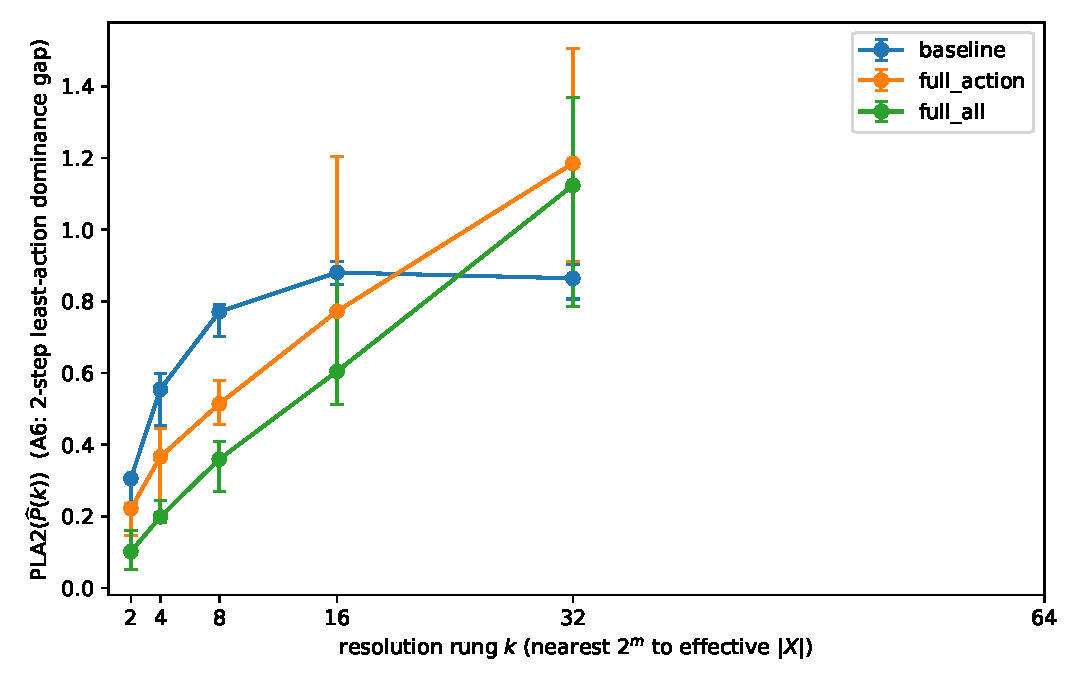
\includegraphics[width=0.49\linewidth]{fig/F4a_PLA2_n128.pdf} &
  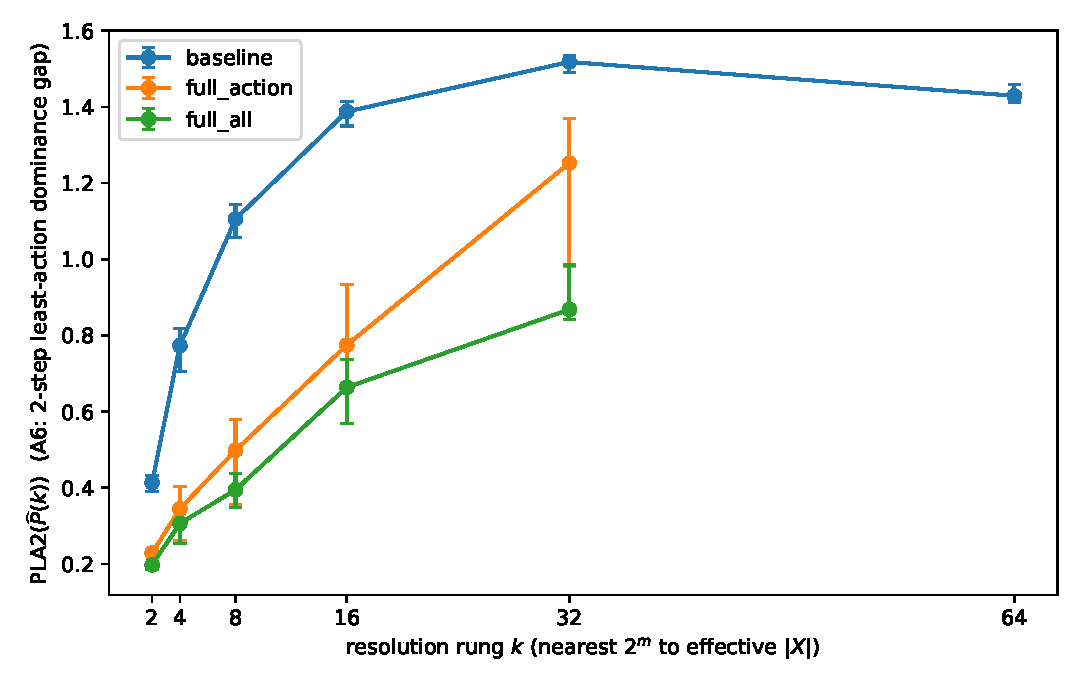
\includegraphics[width=0.49\linewidth]{fig/F4a_PLA2_n256.pdf}\\[0.3em]
  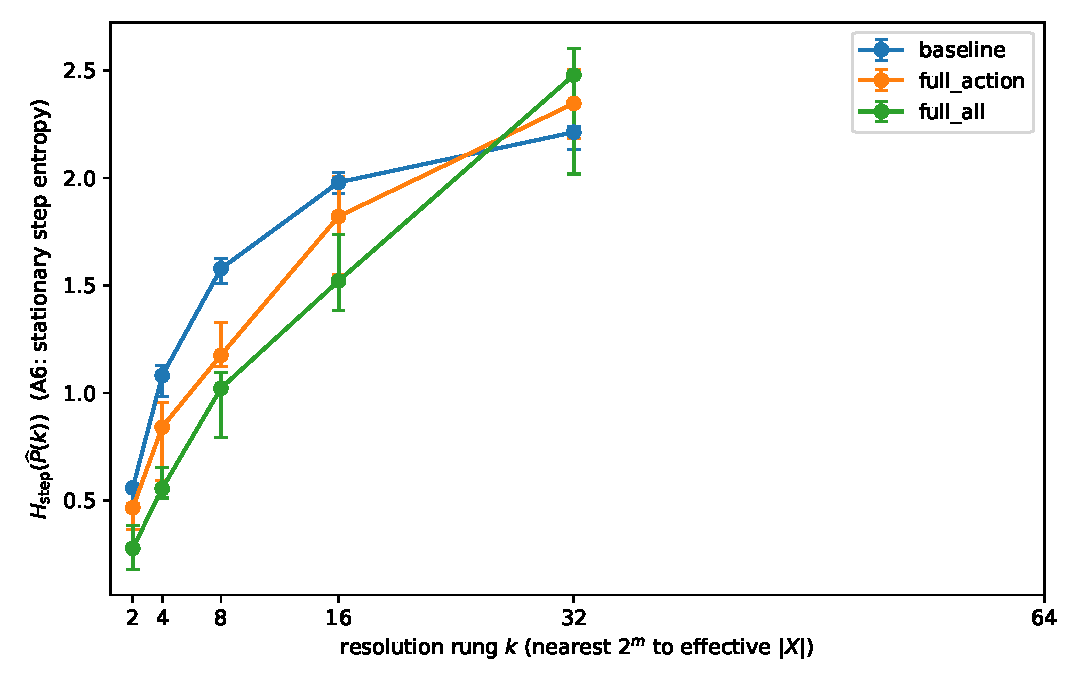
\includegraphics[width=0.49\linewidth]{fig/F4b_step_entropy_n128.pdf} &
  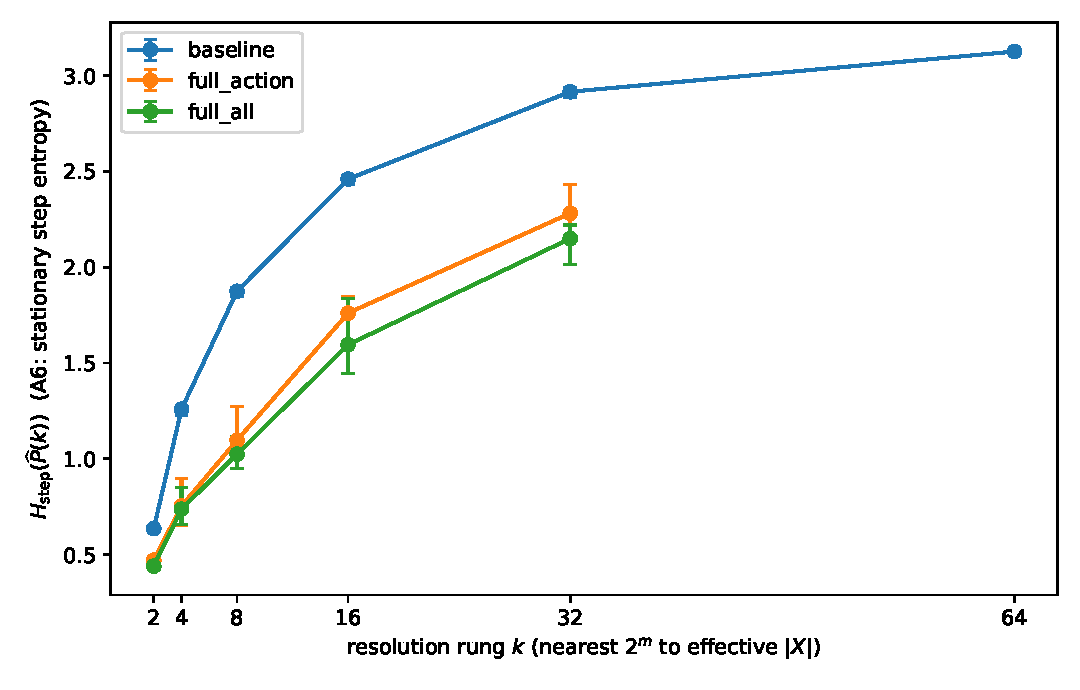
\includegraphics[width=0.49\linewidth]{fig/F4b_step_entropy_n256.pdf}\\[0.3em]
  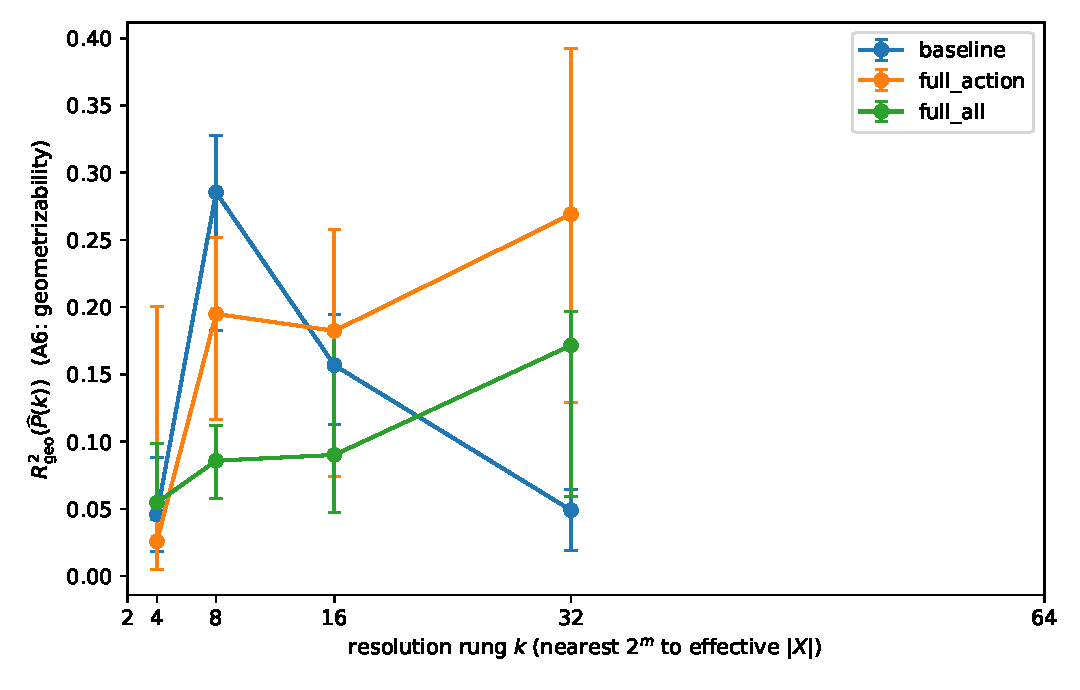
\includegraphics[width=0.49\linewidth]{fig/F4c_geo_r2_n128.pdf} &
  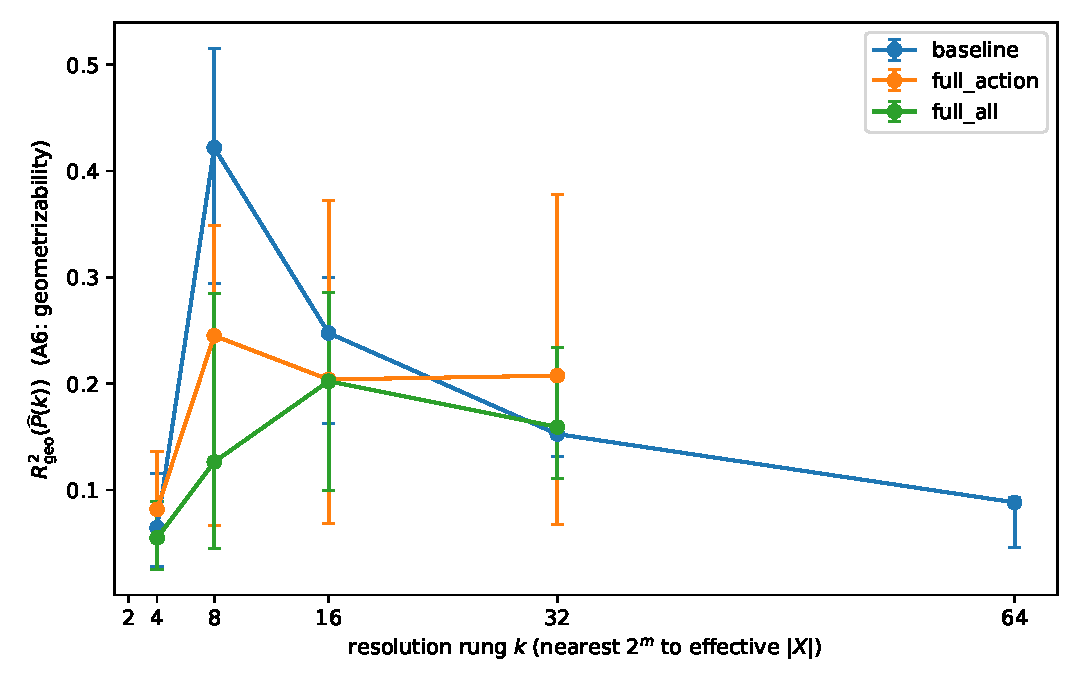
\includegraphics[width=0.49\linewidth]{fig/F4c_geo_r2_n256.pdf}\\[0.3em]
  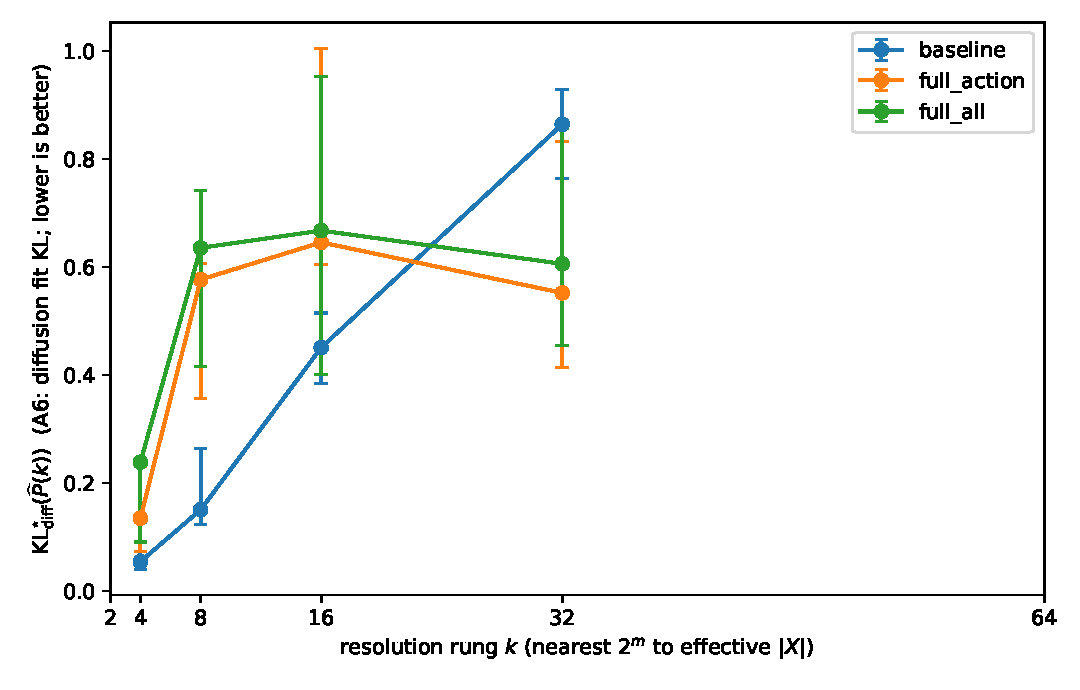
\includegraphics[width=0.49\linewidth]{fig/F4d_diff_kl_n128.pdf} &
  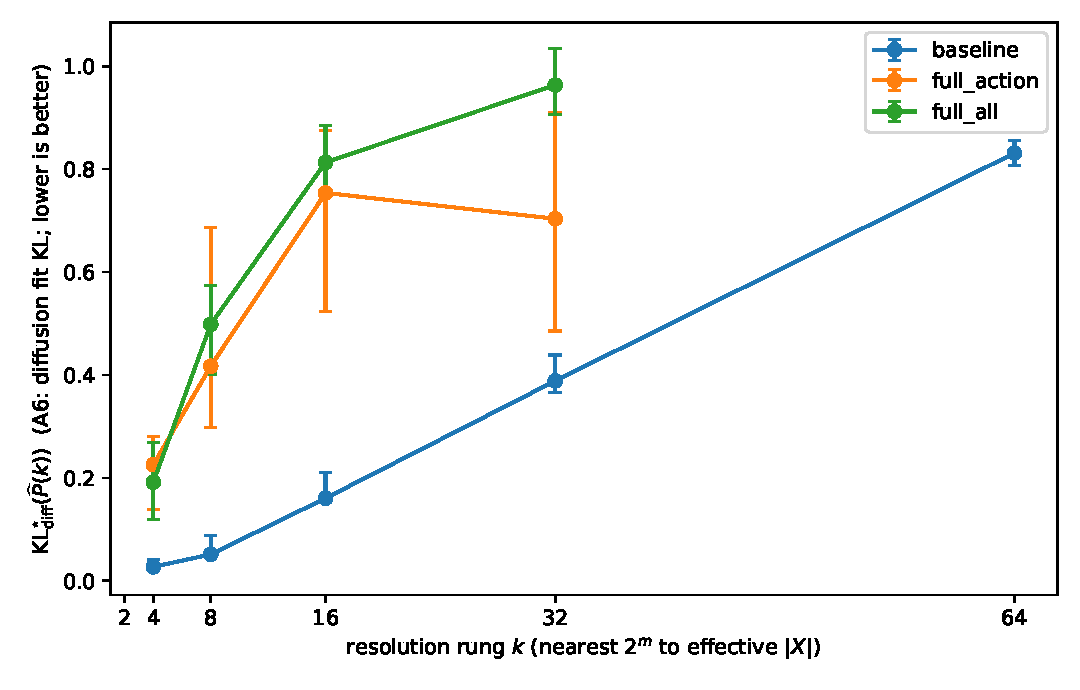
\includegraphics[width=0.49\linewidth]{fig/F4d_diff_kl_n256.pdf}\\
\end{tabular}
\caption{F4: Lagrangian probes vs. resolution for $n=128$ (left) and $n=256$ (right). Rows show: (a) PLA2 gap, (b) step entropy, (c) geometrizability $R^2_{\mathrm{geo}}$, (d) diffusion misfit $\mathrm{KL}^{\star}_{\mathrm{diff}}$. Curves show medians with interquartile ranges; min-support filter (5 seeds) applied. The x-axis uses resolution rung $k$ defined as the nearest power-of-two to effective $k_{\mathrm{eff}}=|\X|$.}
\label{fig:F4_lagrange_n128}
\end{figure}

\subsection{C3: Regime separation across the full ablation suite}
To summarize regime diversity across scales, Figure~\ref{fig:F5_regime_scatter_n128} plots run-level core-rung medians for the full ablation suite at $n=128$ and for the selected scaling suite at $n=256$ in the plane spanned by geometrizability and time-asymmetry.
The full ablation suite occupies a broad region rather than collapsing to a one-dimensional tradeoff, and key conditions (Null/Baseline/Full and compact generators) separate cleanly in this plane, supporting the existence of at least two macroscopic regimes within a single substrate and audit framework.

\begin{figure}[htbp]
\centering
\begin{minipage}[t]{0.49\linewidth}
\centering
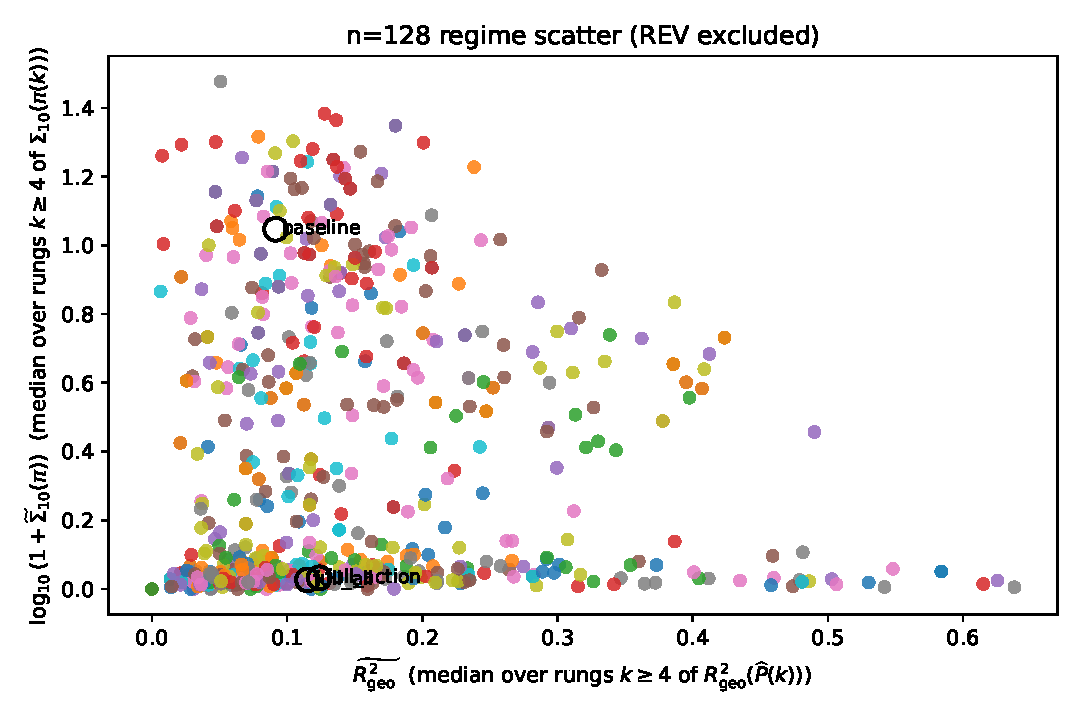
\includegraphics[width=0.98\linewidth]{fig/F5_regime_scatter_n128.pdf}
\end{minipage}\hfill
\begin{minipage}[t]{0.49\linewidth}
\centering
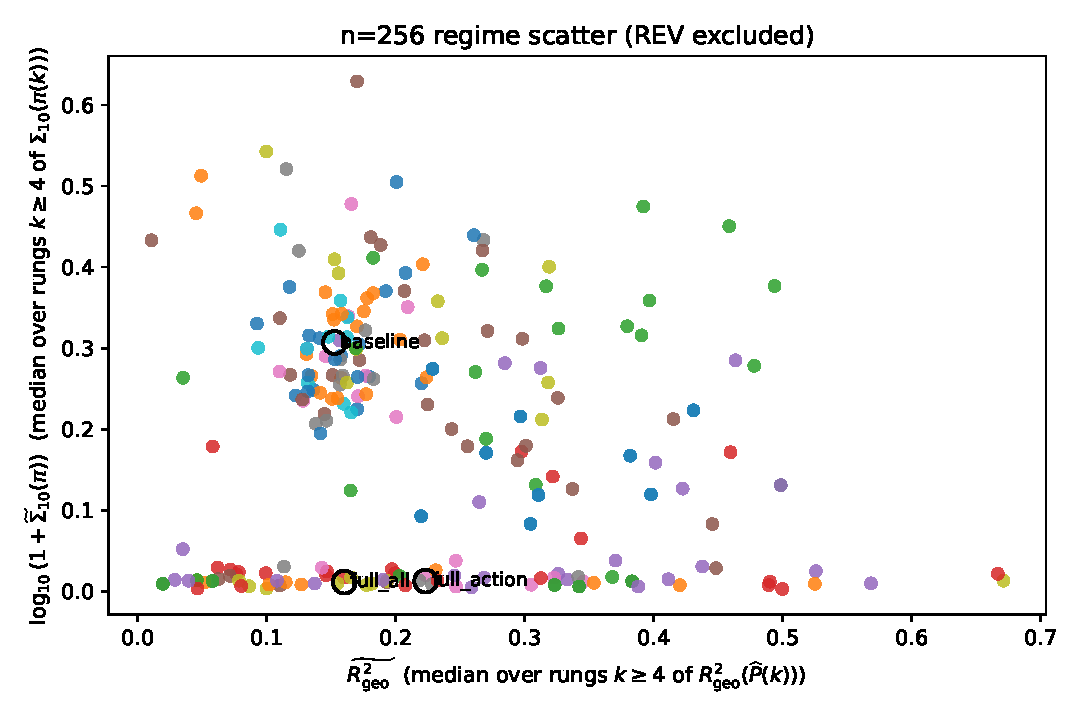
\includegraphics[width=0.98\linewidth]{fig/F5_regime_scatter_n256.pdf}
\end{minipage}
\caption{F5: Regime separation using run-level core-rung medians ($k\ge 4$), with $x=\widetilde{R^2_{\mathrm{geo}}}$ and $y=\log_{10}(1+\widetilde{\Sigma}_{10}(\pi))$. Left: $n=128$ full ablation suite. Right: $n=256$ manifest-defined scaling suite combining controls from EXP-F1/EXP-107 with EXP-112 selective configurations; this right panel therefore has fewer configurations and partial seeds in the EXP-112 selective subset. REV runs are excluded in both panels.}
\label{fig:F5_regime_scatter_n128}
\end{figure}

\subsection{C4: Leave-one-out ablations identify sensitive PICA cells}
Figure~\ref{fig:F6_loo_heatmap} reports leave-one-out (LOO) ablations around Full-Action.
Each column removes exactly one enabled PICA cell while keeping all others fixed, and each row reports the standardized change in a headline metric.
The resulting sensitivity structure is sparse: a small subset of cells produce the largest deviations when removed, indicating candidate generators for specific emergent signatures (geometry-like versus thermodynamic/time-asymmetric).

\begin{figure}[htbp]
\centering
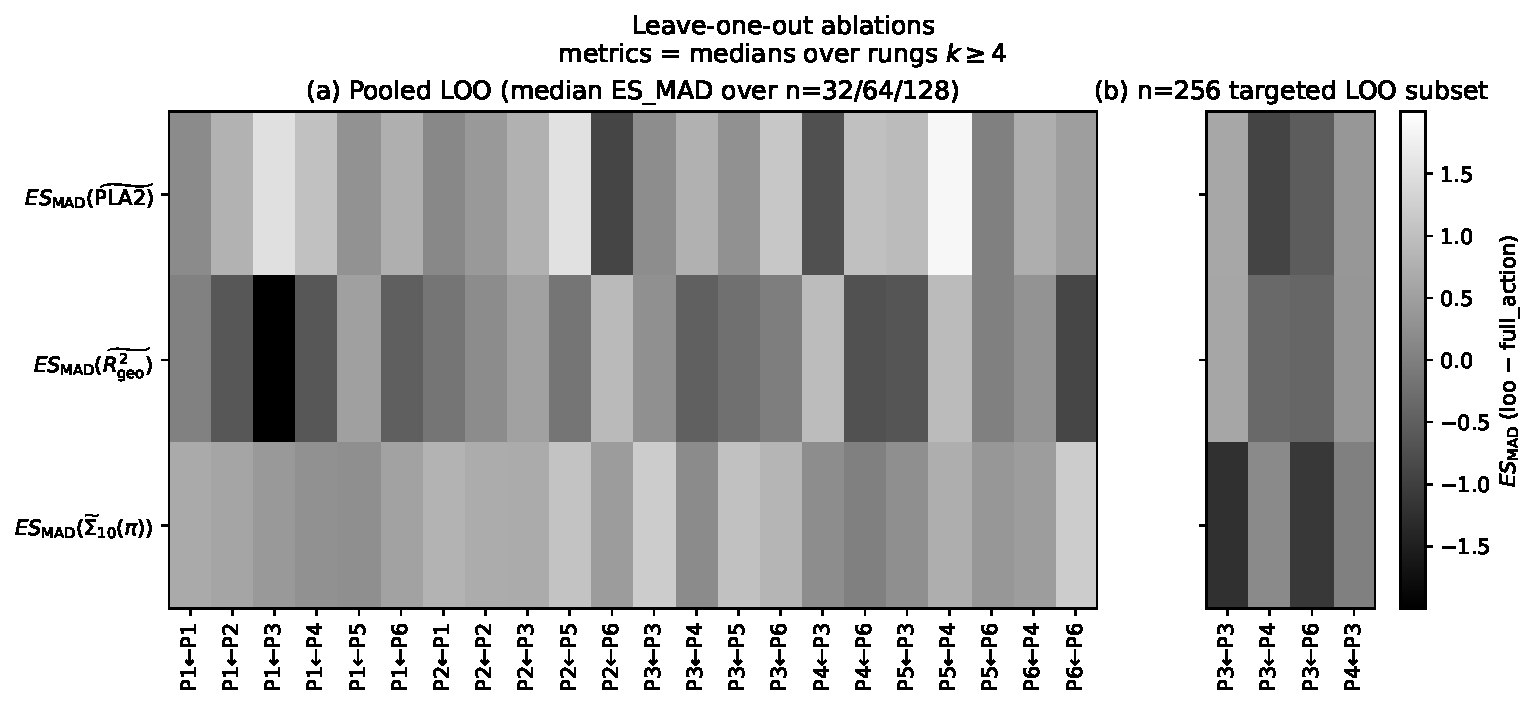
\includegraphics[width=0.90\linewidth]{fig/F6_LOO_heatmap.pdf}
\caption{F6: Leave-one-out ablation sensitivity around Full-Action with two panels. Panel (a) shows the pooled LOO heatmap using the full 22-cell suite over $n\in\{32,64,128\}$ (stratified ES\_MAD pooled by median across sizes). Panel (b) shows the targeted n=256 subset only (available LOO configs), using the same effect-size scale. Columns correspond to removed PICA cells (actor$\leftarrow$informant), and rows correspond to headline metrics (core-rung medians over $k\ge 4$).}
\label{fig:F6_loo_heatmap}
\end{figure}

\subsection{C5: Probe couplings at anchor rung $k=4$ are strong and size-dependent}
Table~\ref{tab:T5A_correlations} reports Spearman correlations among Lagrange probes at the anchor rung $k=4$ across all configurations and seeds, stratified by $n$ (REV excluded).
Two robust patterns emerge.
First, PLA2 gap and step entropy are almost collinear across sizes ($\rho\approx 0.97$ for all $n$), showing that action-consistency and transition stochasticity are tightly coupled at the anchor scale.
Second, the relationships between (PLA2, step entropy) and geometry/diffusion probes change substantially with $n$, indicating that the probe manifold itself evolves with micro size at fixed anchor resolution.
The $n=256$ correlations are computed on the manifest-defined scaling suite (26 configurations) and should therefore be read as a targeted consistency check rather than a like-for-like replacement of the full $n=128$ ablation suite.

\subsection{C6: Partition competition increases diffusion misfit at $k=4$}
Table~\ref{tab:T5B_regression} tests a fixed regression of diffusion misfit at $k=4$ against membership in a predefined partition-competition subset (Methods; REV excluded).
At $n=32$, $n=128$, and $n=256$ the estimated effect is positive with bootstrap confidence intervals excluding zero, indicating systematically higher diffusion misfit for that subset at the anchor rung; at $n=64$ the confidence interval crosses zero (Table~\ref{tab:T5B_regression}).

\subsection{Robustness outcome panels}
Figure~\ref{fig:F7_tau_distribution} and Figure~\ref{fig:F8_sigma_ratio_distribution} summarize the robustness outcomes across sizes, including $n=256$.

\begin{figure}[htbp]
\centering
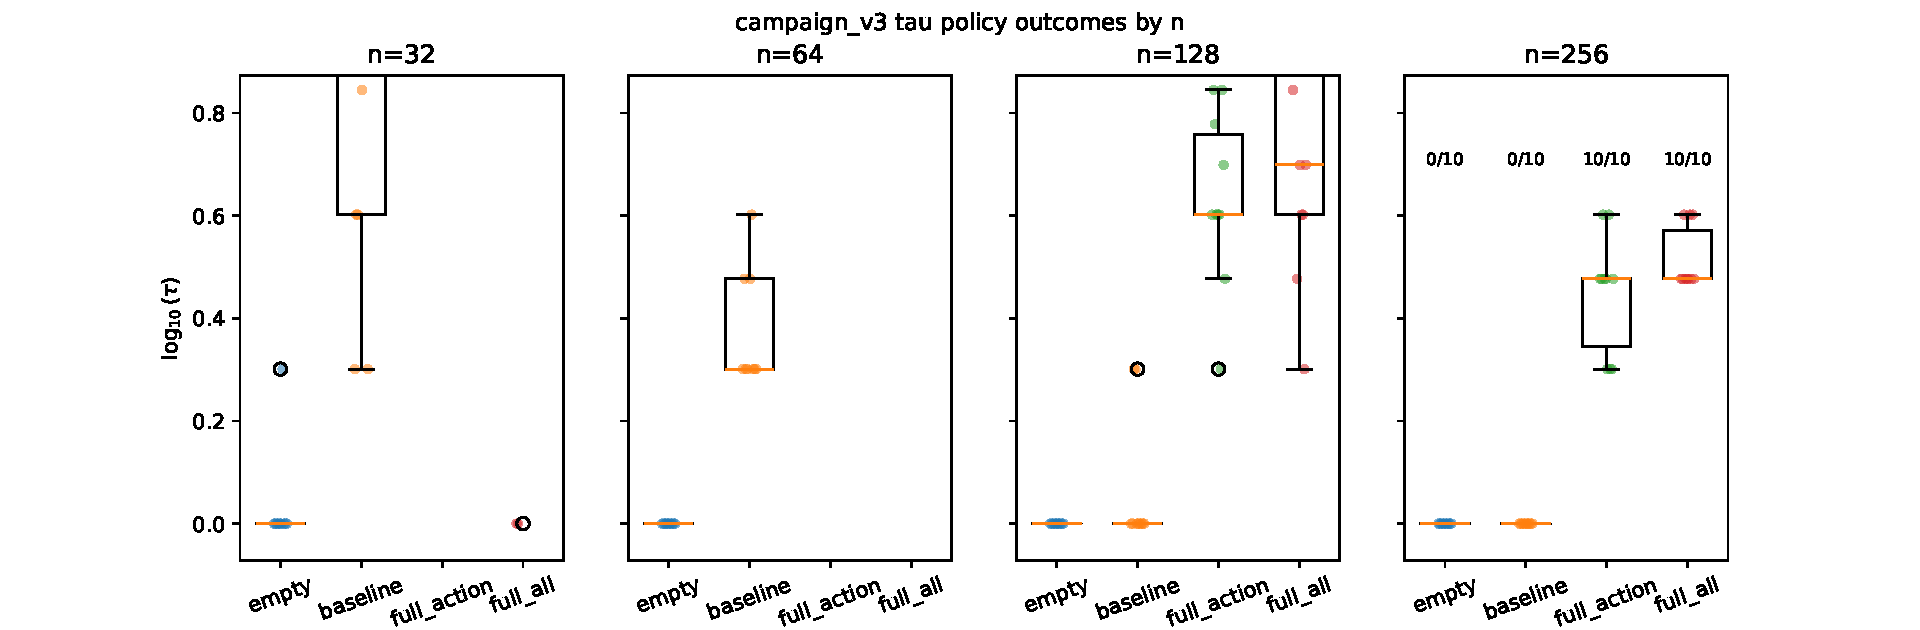
\includegraphics[width=0.92\linewidth]{fig/F7_tau_distribution.pdf}
\caption{F7: Timescale-policy outcome distributions across $n\in\{32,64,128,256\}$ for key conditions (empty, baseline, full\_action, full\_all). The plotted quantity is $\log_{10}(\tau)$, and per-condition annotations report active-$\tau$ availability counts.}
\label{fig:F7_tau_distribution}
\end{figure}

\begin{figure}[htbp]
\centering
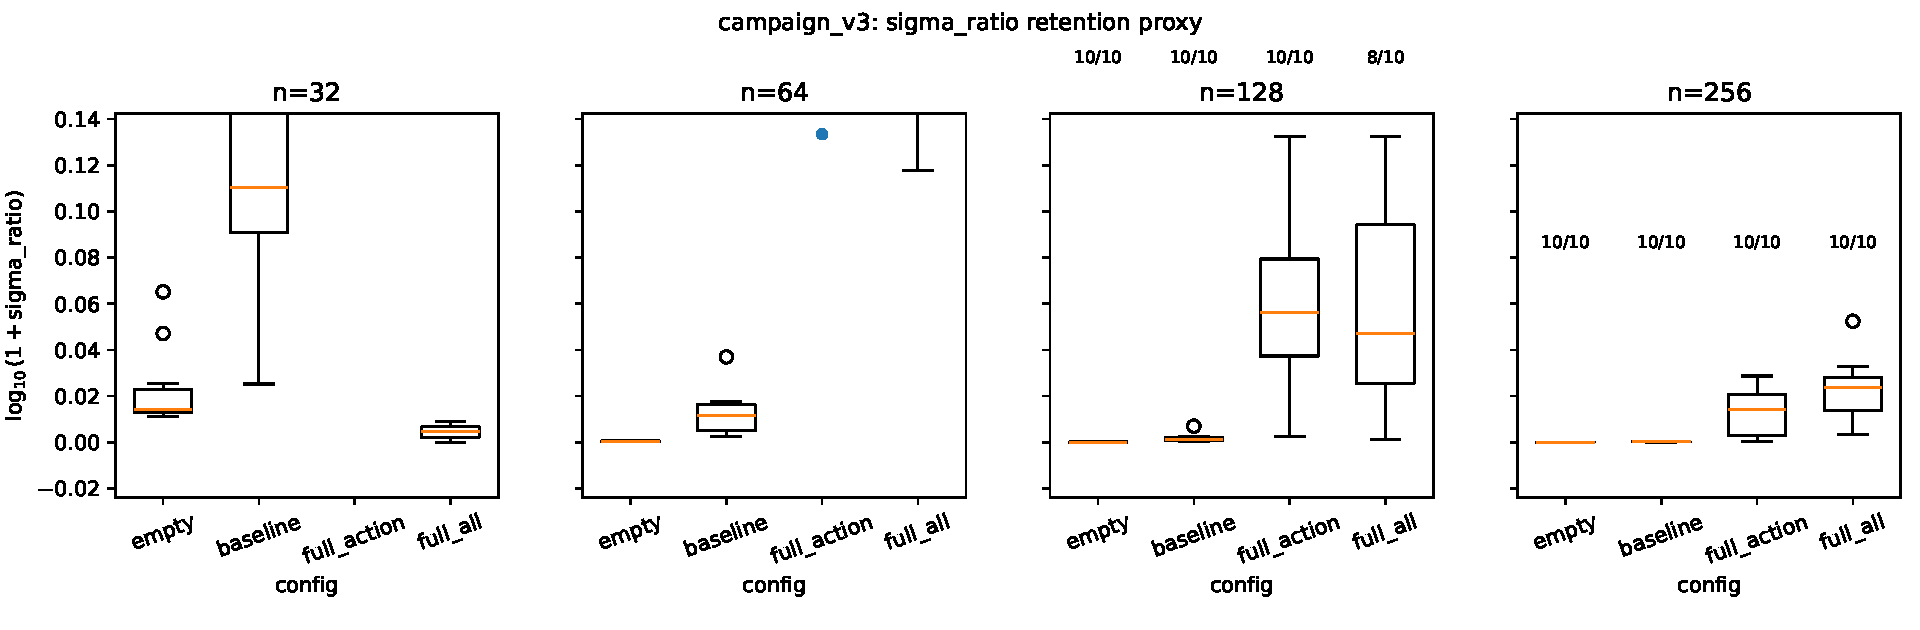
\includegraphics[width=0.95\linewidth]{fig/F8_sigma_ratio_distribution.pdf}

\medskip
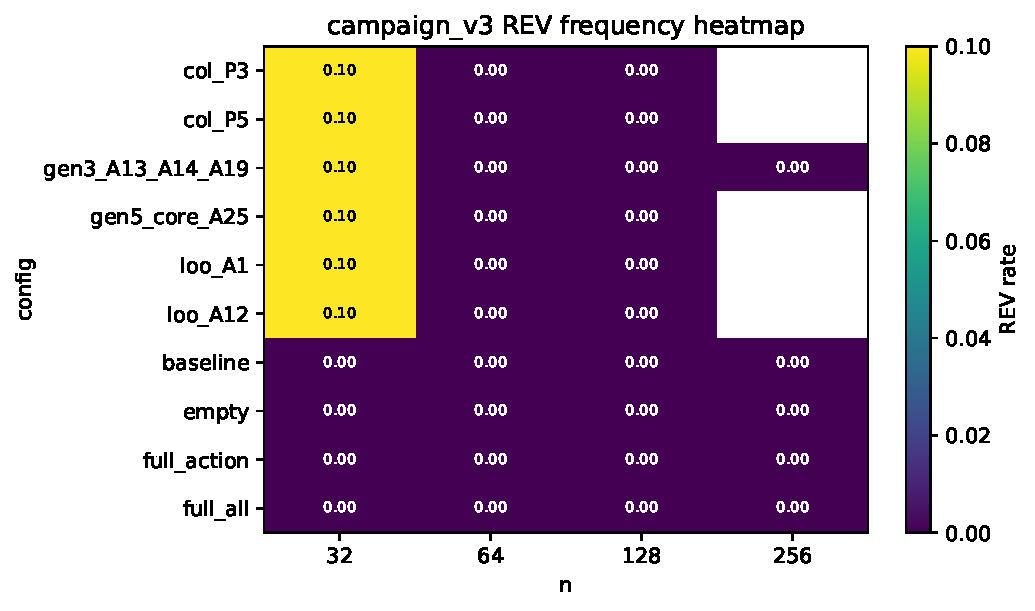
\includegraphics[width=0.65\linewidth]{fig/F8_REV_frequency_heatmap.pdf}
\caption{F8: Robustness diagnostics across $n\in\{32,64,128,256\}$. Top: EP-retention proxy distribution using $\log_{10}(1+\sigma_{\mathrm{ratio}})$ for key conditions, with explicit defined-count annotations. Bottom: REV frequency heatmap (REV rate) by configuration and size.}
\label{fig:F8_sigma_ratio_distribution}
\end{figure}

% Auto-generated by paper/scripts/build_T5_correlations_regression.py
% Auto-generated by paper/scripts/build_T5_correlations_regression.py
\begin{table*}[t]
\scriptsize
\centering
\caption{T5A: Spearman correlations among Lagrange probes at anchor rung $k=4$ (REV excluded), with BH-FDR correction per $n$ over 6 tests. p-values computed by SciPy or deterministic 5000-permutation fallback.}
\label{tab:T5A_correlations}
\begin{tabular}{l l r r r r}
\toprule
$n$ & Pair & $\rho$ & $p$ & $q$ & $N$ \\
\midrule
\multicolumn{6}{l}{\textbf{$n=32$}} \\
32 & $\mathrm{PLA2}\leftrightarrow H_{\mathrm{step}}$ & 0.973 & 0 & 0 & 684 \\
32 & $\mathrm{PLA2}\leftrightarrow R^2_{\mathrm{geo}}$ & -0.451 & 1.29e-28 & 1.55e-28 & 543 \\
32 & $\mathrm{PLA2}\leftrightarrow \mathrm{KL}^{\star}_{\mathrm{diff}}$ & 0.701 & 1.83e-81 & 3.65e-81 & 544 \\
32 & $H_{\mathrm{step}}\leftrightarrow R^2_{\mathrm{geo}}$ & -0.417 & 2.94e-24 & 2.94e-24 & 543 \\
32 & $H_{\mathrm{step}}\leftrightarrow \mathrm{KL}^{\star}_{\mathrm{diff}}$ & 0.783 & 6.07e-114 & 1.82e-113 & 544 \\
32 & $R^2_{\mathrm{geo}}\leftrightarrow \mathrm{KL}^{\star}_{\mathrm{diff}}$ & -0.473 & 1.2e-31 & 1.8e-31 & 543 \\
\midrule
\multicolumn{6}{l}{\textbf{$n=64$}} \\
64 & $\mathrm{PLA2}\leftrightarrow H_{\mathrm{step}}$ & 0.972 & 0 & 0 & 690 \\
64 & $\mathrm{PLA2}\leftrightarrow R^2_{\mathrm{geo}}$ & -0.146 & 0.000181 & 0.000181 & 649 \\
64 & $\mathrm{PLA2}\leftrightarrow \mathrm{KL}^{\star}_{\mathrm{diff}}$ & 0.257 & 2.84e-11 & 4.26e-11 & 649 \\
64 & $H_{\mathrm{step}}\leftrightarrow R^2_{\mathrm{geo}}$ & -0.188 & 1.36e-06 & 1.63e-06 & 649 \\
64 & $H_{\mathrm{step}}\leftrightarrow \mathrm{KL}^{\star}_{\mathrm{diff}}$ & 0.266 & 6.17e-12 & 1.23e-11 & 649 \\
64 & $R^2_{\mathrm{geo}}\leftrightarrow \mathrm{KL}^{\star}_{\mathrm{diff}}$ & -0.443 & 1.62e-32 & 4.87e-32 & 649 \\
\midrule
\multicolumn{6}{l}{\textbf{$n=128$}} \\
128 & $\mathrm{PLA2}\leftrightarrow H_{\mathrm{step}}$ & 0.975 & 0 & 0 & 690 \\
128 & $\mathrm{PLA2}\leftrightarrow R^2_{\mathrm{geo}}$ & 0.306 & 1.96e-16 & 2.36e-16 & 689 \\
128 & $\mathrm{PLA2}\leftrightarrow \mathrm{KL}^{\star}_{\mathrm{diff}}$ & -0.715 & 4.33e-109 & 1.3e-108 & 689 \\
128 & $H_{\mathrm{step}}\leftrightarrow R^2_{\mathrm{geo}}$ & 0.242 & 1.28e-10 & 1.28e-10 & 689 \\
128 & $H_{\mathrm{step}}\leftrightarrow \mathrm{KL}^{\star}_{\mathrm{diff}}$ & -0.71 & 7.73e-107 & 1.55e-106 & 689 \\
128 & $R^2_{\mathrm{geo}}\leftrightarrow \mathrm{KL}^{\star}_{\mathrm{diff}}$ & -0.31 & 8.83e-17 & 1.32e-16 & 689 \\
\midrule
\multicolumn{6}{l}{\textbf{$n=256$}} \\
256 & $\mathrm{PLA2}\leftrightarrow H_{\mathrm{step}}$ & 0.994 & 1.74e-228 & 1.04e-227 & 237 \\
256 & $\mathrm{PLA2}\leftrightarrow R^2_{\mathrm{geo}}$ & 0.205 & 0.00155 & 0.00232 & 237 \\
256 & $\mathrm{PLA2}\leftrightarrow \mathrm{KL}^{\star}_{\mathrm{diff}}$ & -0.827 & 8.69e-61 & 1.74e-60 & 237 \\
256 & $H_{\mathrm{step}}\leftrightarrow R^2_{\mathrm{geo}}$ & 0.15 & 0.0208 & 0.0249 & 237 \\
256 & $H_{\mathrm{step}}\leftrightarrow \mathrm{KL}^{\star}_{\mathrm{diff}}$ & -0.831 & 9.18e-62 & 2.75e-61 & 237 \\
256 & $R^2_{\mathrm{geo}}\leftrightarrow \mathrm{KL}^{\star}_{\mathrm{diff}}$ & -0.0775 & 0.235 & 0.235 & 237 \\
\bottomrule
\end{tabular}
\end{table*}

\begin{table}[t]
\scriptsize
\centering
\caption{T5B: OLS regression by $n$ at $k=4$ (REV excluded): $\mathrm{KL}^{\star}_{\mathrm{diff}}(k{=}4)\sim 1 + \mathbb{I}[\mathrm{competition}]$. $\beta_1$ is competition$-$noncompetition. 95\% CI from bootstrap ($B=5000$).}
\label{tab:T5B_regression}
\begin{tabular}{r r r r r r}
\toprule
$n$ & $\beta_1$ & 95\% CI & $N_{\mathrm{total}}$ & $N_{\mathrm{comp}}$ & $N_{\mathrm{noncomp}}$ \\
\midrule
32 & 0.0274 & [0.00251, 0.0517] & 544 & 43 & 501 \\
64 & 0.0124 & [-0.00633, 0.0328] & 649 & 48 & 601 \\
128 & 0.0293 & [0.0143, 0.043] & 689 & 50 & 639 \\
256 & 0.0968 & [0.0554, 0.138] & 237 & 21 & 216 \\
\bottomrule
\end{tabular}
\end{table}



\section{Discussion}
\label{sec:discussion}

\subsection{Interpretation: regimes rather than a single macroscopic behavior}
The multiscale audits show that a single minimal stochastic substrate on $\Z$ can support a wide range of macroscopic behaviors once closure is enabled through PICA.
Two qualitative patterns recur across figures and tables.
First, Full-Action/Full-All reorganize the multiscale structure of induced kernels $\Phat(k)$ (Fig.~\ref{fig:F3_multiscale}) and strongly suppress macro path-reversal asymmetry as quantified by $\Sigma_{10}(\pi)$ (Table~\ref{tab:T3_headline_metrics}).
Second, the Lagrangian probes reveal that geometry/diffusion consistency is not a monotone function of resolution: for $n=128$ (full suite) and $n=256$ (scaling suite), $R^2_{\mathrm{geo}}$ and $\mathrm{KL}^{\star}_{\mathrm{diff}}$ shift markedly along the ladder (Fig.~\ref{fig:F4_lagrange_n128}), and the resulting run-level medians separate into distinct regions in the $(\widetilde{R^2_{\mathrm{geo}}},\log_{10}(1+\widetilde{\Sigma}_{10}(\pi)))$ plane (Fig.~\ref{fig:F5_regime_scatter_n128}).

A natural interpretation is therefore \emph{regimes} (or universality-class-like behavior) rather than a single emergent macro law.
In the present audits, one regime is ``geometry-like'' in the operational sense that transition actions correlate with squared embedding distances and diffusion-kernel fits improve at finer resolutions; another regime is ``thermodynamic/\allowbreak{}time-asymmetric'' in the operational sense that stationary path-reversal asymmetry and cycle-affinity diagnostics become prominent.
We emphasize that these are \emph{audit-defined} regimes, not claims of literal spacetime geometry or physical thermodynamics in the microscopic substrate.
They are nonetheless useful because they tie specific macroscopic signatures to specific closure mechanisms and ablation subalgebras, in a way that is legible to statistical mechanics readers \cite{Anderson1972,WilsonKogut1974,Seifert2012,Esposito2012CoarseGraining}.

\subsection{PICA as a reusable closure interaction algebra}
A key contribution of this work is to separate ``what emerges'' from ``how closure is specified''.
PICA, represented by $\Epica\in\{0,1\}^{6\times6}$, provides a canonical interaction grammar for closure: it makes the space of mechanisms explicit (36 directed cells) and makes ablations compositional (subsets $S\subseteq\mathrm{PICA}$, subject to closure/\allowbreak{}dependency constraints).
The leave-one-out analysis (Fig.~\ref{fig:F6_loo_heatmap}) suggests that sensitivity is structured rather than diffuse: removing certain cells produces large, metric-specific deviations, while many removals have modest effects.
This motivates the view that macroscopic regimes can have \emph{generators}: small cell sets that are sufficient (within this substrate and scan protocol) to elicit strong geometry-like or thermodynamic/time-asymmetric signatures.

At the same time, the current LOO family probes only cells that can be removed without breaking essential scaffolding; in particular, two Full-Action-enabled cells (the spectral partition core and its coupled gating) were not included as single-removal LOO configurations.
Thus the sensitivity pattern should be interpreted as \emph{conditional on the present pipeline} rather than a universal ranking of cell importance.

\subsection{Coarse-graining pitfalls and ``no smuggling''}
Because our conclusions are based on induced macro kernels $\Phat = U_f P^\tau Q_f$, they inherit the well-known ambiguity of coarse-graining: different lenses $f$ can yield different macrodynamics, and aggregation can conceal dissipation or introduce apparent irreversibility artifacts \cite{Esposito2012CoarseGraining,KawaguchiNakayama2013}.
We therefore treat the audits as \emph{detectors} (operational tests) rather than direct measurements of physical quantities.
Three examples illustrate the general point.

First, $\Sigma_{10}(\pi)$ is a time-asymmetry proxy computed from the ratio $\Phat_{ij}/\Phat_{ji}$ and is sensitive to numerical floors/caps when one direction is near-zero.
Second, least-action dominance (PLA2) depends on the action surrogate $\ell=-\log \Phat_{ij}$ with an $\varepsilon$ floor, so it can be influenced by rare-transition regularization.
Third, geometrizability and diffusion-fit quality are defined through a reversible embedding of $\Phat$ and therefore can fail or become ill-conditioned for small $k$ or degenerate stationary mass; these cases appear as missing values and motivate interpreting $R^2_{\mathrm{geo}}$ and $\mathrm{KL}^{\star}_{\mathrm{diff}}$ as conditional diagnostics rather than universal invariants.
The value of the present pipeline is that these detectors are defined explicitly (Methods) and are applied systematically across subalgebras, sizes, and seeds.

\subsection{Limitations and falsifiability}
The following limitations are explicit constraints on what the present experiments can support, and they also define concrete falsifiers for the claims in the Results section.

\paragraph{Limitations and confounds (A6-consistent).}
\begin{itemize}
  \item \textbf{Finite-size scope and selective scaling.} We evaluate only $n\in\{32,64,128,256\}$, and the $n=256$ data are a selected scaling suite rather than the full 69-configuration ablation set. Asymptotic scaling trends are therefore not established, and any size-dependent statements should be interpreted as finite-size evidence within a manifest-defined experimental design.
  \item \textbf{Lens dependence.} The multiscale ladder uses a specific spectral sign-pattern partition construction; alternative lens families or alternative lifts $Q_f$ could shift (or erase) observed regimes. This is a structural coarse-graining confound.
  \item \textbf{Adaptive timescale coupling.} The timescale $\tau$ is not held fixed across conditions. In particular, direct $\tau$-matched comparisons between Baseline and Full-Action are not broadly available in the current dataset (see robustness checklist), which limits causal attribution of differences solely to closure cells.
  \item \textbf{Macro thermodynamics is not micro thermodynamics.} $\Sigma_{10}(\pi)$ and related cycle diagnostics are macro-level proxies; they do not, by themselves, quantify micro-level entropy production. Hidden dissipation under coarse-graining is a known pitfall \cite{Esposito2012CoarseGraining}.
  \item \textbf{Numerical regularization.} Several audits use numerical floors/caps (e.g., $\varepsilon$ in $-\log$ action; caps for near-zero reverse transitions). These stabilize computation but can bias extreme-tail behavior.
  \item \textbf{Probe missingness.} Geometry and diffusion probes can be undefined for certain rungs (embedding degeneracy). Missingness is explicitly tracked, but it reduces effective sample size for those probes at some scales.
  \item \textbf{Partial ablation coverage.} The LOO family does not include all Full-Action-enabled cells; two core spectral cells are not tested by single-removal LOO, so generator claims are conditional.
\end{itemize}

\paragraph{What would falsify our claim framing (A9.1-style).}
\begin{itemize}
  \item \textbf{C1 falsifier:} If additional seeds or reruns remove the Full vs Baseline separation in headline time-asymmetry and structure (Table~\ref{tab:T3_headline_metrics}) once $\tau$ is controlled or matched, then the ``full PICA reshapes macro behavior'' interpretation would weaken substantially.
  \item \textbf{C2 falsifier:} If the geometry/diffusion improvements at fine resolution (Fig.~\ref{fig:F4_lagrange_n128}) disappear under alternative coarse-graining procedures or alternative lifts $Q_f$, then the geometry-like regime would be better viewed as a property of the chosen lens rather than the closure dynamics.
  \item \textbf{C3 falsifier:} If the regime scatter (Fig.~\ref{fig:F5_regime_scatter_n128}) collapses under minor audit-parameter changes (e.g., path horizon $T$ for $\Sigma_{10}(\pi)$, embedding dimension $m$), then the ``multiple regimes'' story would need to be revised.
  \item \textbf{C4 falsifier:} If LOO sensitivity patterns (Fig.~\ref{fig:F6_loo_heatmap}) are unstable across seeds/sizes or disappear when the two untested spectral cells are included in ablations, then the ``generator'' interpretation would be unsupported.
  \item \textbf{C5--C6 falsifier:} If the anchor-rung correlations and the competition-family regression (Table~\ref{tab:T5A_correlations}, Table~\ref{tab:T5B_regression}) fail to replicate under strict REV handling and multiple-testing controls, then the probe-coupling and competition effect claims should be treated as exploratory.
\end{itemize}

\subsection{Future work}
Several follow-on experiments would strengthen both the physics-like narrative and the algebraic/PICA contribution.

\begin{itemize}
  \item \textbf{Controlled-$\tau$ reruns.} Run matched-$\tau$ sweeps (or fixed-$\tau$ protocols) for Baseline vs Full conditions to separate closure effects from timescale effects.
  \item \textbf{Alternative lenses and lifts.} Repeat the multiscale scan with alternative coarse-graining constructions (e.g., different spectral clustering variants) and non-uniform lifts $Q_f$ (e.g., conditional stationary lifts) to test lens robustness.
  \item \textbf{Scaling.} Extend to larger $n$ and larger $k$ ladders, and test whether the regime separation sharpens, merges, or transitions.
  \item \textbf{Ablation completion.} Add ablations that remove the two currently untested spectral core cells (or replace them with alternative partition primitives) to complete the generator picture.
  \item \textbf{Audit stress tests.} Vary path horizon $T$, embedding dimension $m$, and regularization floors to quantify audit stability and reduce confounds.
  \item \textbf{Cross-substrate transfer.} Apply the disciplined PICA cell catalog to other substrates. The six primitives have been used on particle-based and neural/meta-layer toy substrates \cite{Tsiokos2026Life}, but with additional non-PICA mechanisms; re-implementing those substrates under strict PICA closure would test whether similar regimes emerge without extra assumptions and whether generator subalgebras transfer.
\end{itemize}

\section{Conclusion}
\label{sec:conclusion}

We presented a minimal stochastic substrate together with a coarse-graining pipeline and a six-primitive closure interaction algebra (PICA) that enables systematic, compositional ablations over a 6$\times$6 directed interaction table.
Across an exhaustive ablation suite at $n\in\{32,64,128\}$ (2070 runs over 69 PICA subalgebras) together with a selected scaling suite at $n=256$ (237 runs), totaling 2307 runs, exhaustive activation and structured ablations produce robust, scale-dependent macroscopic signatures in induced kernels $\Phat(k)$ that are operationally consistent with distinct regimes: geometry/diffusion-like structure at fine resolution and thermodynamic/time-asymmetric structure in other parts of configuration space.
The scaling suite provides an additional large-$n$ consistency check for controls and targeted mechanisms without changing the qualitative claim structure established by the exhaustive suite.
The key point is not that the substrate literally contains spacetime or thermodynamics, but that a single Markov audit framework can detect lawfulness-like structure that tracks specific closure mechanisms.

Beyond the toy-universe results, PICA functions as a reusable object: a canonical interaction grammar for closure that can be instantiated on other substrates and compared via a shared ablation calculus.

\section*{CRediT authorship contribution statement}
Ioannis A.: Conceptualization; Methodology; Software; Formal analysis; Investigation; Validation; Visualization; Writing -- original draft; Writing -- review \& editing.

\section*{Declaration of competing interest}
The author declares that there are no known competing financial interests or personal relationships that could have appeared to influence the work reported in this paper.

\section*{Funding}
This research did not receive any specific grant from funding agencies in the public, commercial, or not-for-profit sectors.
% TODO: Replace with actual funder/grant information if applicable.

\section*{Data availability}
Source code is available at \url{https://github.com/ioannist/six-birds-pica}.
The code, configurations, and processed run artifacts required to reproduce the figures and tables will be deposited as a reproducibility package in the Mendeley Data repository (DOI: TBD).
The deposit will include a frozen code snapshot, experiment configurations and seeds, per-run audit outputs, derived analysis tables, and scripts to regenerate all figures and tables.

\section*{Declaration of generative AI use}
The author used AI assistants (OpenAI GPT-5.2 Pro, Anthropic Claude) to help draft text, organize structure, and generate code snippets.
All content was reviewed, verified, and edited by the author, who takes full responsibility for the published article.
All figures were produced programmatically from the deposited data.

\section*{Acknowledgements}
% TODO: Add acknowledgements (individuals, institutions, discussions, proofreading) if applicable.

% References (BibTeX)
\bibliographystyle{unsrt}
\bibliography{references}

\end{document}
